\documentclass{article}
\usepackage[utf8]{inputenc}
\usepackage[maxcitenames=1,style=numeric]{biblatex}
\usepackage{amsmath}
\usepackage{amssymb}
\usepackage{amsthm}
\usepackage{tcolorbox}
\usepackage{graphicx}
\usepackage{algorithm}
\usepackage{algorithmic}
\usepackage{hyperref}
\usepackage{cleveref}
\usepackage{thmtools}
\usepackage{thm-restate}
\usepackage{enumerate}
\usepackage{xcolor}
\usepackage{textgreek}
\usepackage{caption}
\usepackage{subcaption}
\usepackage{authblk}
% \usepackage[table,xcdraw]{xcolor}
% \usepackage{subfloat}

\topmargin -.5in
\textheight 9in
\oddsidemargin -.25in
\evensidemargin -.25in
\textwidth 7in


\newcommand{\cheng}[1]{\textcolor{purple}{{\bf Cheng:~}#1}}
\newcommand{\mengyan}[1]{\textcolor{magenta}{#1}}
\newcommand{\maciej}[1]{\textcolor{blue}{#1}}

% \captionsetup[subfigure]{position=top, labelfont=bf,textfont=normalfont,singlelinecheck=off,justification=raggedright}
\captionsetup[subfigure]{font={bf,small}, skip=1pt, singlelinecheck=false}
\renewcommand{\thesubfigure}{\Alph{subfigure}}

\addbibresource{ref.bib}

\title{Machine Learning guided workflow for Ribosome Binding Site engineering}

\author[1,2,4]{Zhang M.}
\author[3]{Holowko M. B.}
\author[3]{Hayman Zumpe H.}
\author[1,2,4]{Ong, C. S.}
\affil[1]{Machine Learning and Artificial Intelligence Future Science Platform, CSIRO}
\affil[2]{Department of Computer Science, Australian National University}
\affil[3]{CSIRO Synthetic Biology Future Science Platform, CSIRO Land and Water}
\affil[4]{Data61, CSIRO}

\date{\today{}}

\bibliography{ref.bib}
% \DeclareUnicodeCharacter{2212}{-}
\begin{document}

\maketitle

\section*{Abstract}

Fine control of gene expression can be achieved through engineering transcriptional and translation control elements, including the Ribosome Binding Site (RBS).
Unfortunately, RBSs are not understood at the level of finesse required for reliable design. 
To address this problem, we have created a machine learning (ML) enabled workflow for the design of bacterial RBSs.
We used Gaussian Process Regression for prediction and the Upper Confidence Bound-based Bandit algorithm for recommendation of genetic designs to be tested in vitro.
We have integrated the ML algorithms with laboratory automation and high-throughput processes, creating a robust workflow for the design of custom RBSs.
Using our workflow, we generated a novel library of diverse RBSs with a wide range of expression levels.
Notably, a high number of these sites demonstrate translation initiation rates equalling or exceeding the currently known strong RBSs.

\section{Introduction}

One of the main tenets of synthetic biology is design, evaluation and standardisation of genetic parts \cite{Brophy2014,Canton2008,Stanton2014}.
This is usually done in terms of the Design-Build-Test-Learn (DBTL) cycle, where the given genetic part or organism are continually improved by going through a number of turns of the said cycle.
This normally involves designing the DNA sequence in Computer Aided Design (CAD) software and then physically testing it in a laboratory. 
Additionally, computer modelling and prediction of part behaviour based on the designed DNA sequence or design of DNA sequence based on expected function can be used \cite{Yeoh2019,Nielsen2016}.
Most of these models are based on either the thermodynamic properties of the involved molecules (DNA, RNA, proteins, etc.) or empirically obtained values describing a relevant to a given design property, like Translation Initiation Rate (TIR) in the case of Ribosome Binding Sites (RBS) \cite{Xia1998,Chen2013,Reeve2014}.
However, de-novo design of small genetic elements is still challenging due to unknown relationships between sequence and performance of such elements. 
This means that many designers have to rely on known and characterised parts that may not be optimal for their constructs.
The problem with this approach is that such part libraries can also be unreliable due to poor reliability of methods used to obtain them.

The biggest limitation for the DBTL approach currently is the Learn part of the cycle - there is very limited access to methods and software that can improve and understand designs based on the experimental results.
For example, according to  \textcite{Reeve2014} there are three main RBS calculators, all predicting the TIR based on the thermodynamic properties of the RBS and the ribosome \cite{Seo2013,Na2010,Salis2009}. 
Reported predictions from all of these models are relatively good ($R^2 >0.8$), 
% \mengyan{Maciej: reviewer might wonder why they got high R2 but we don't, e.g. is that because the data? So I recommend either remove this or explain it somewhere.} \maciej{I'll explain it in the discussion}
but they come with a number of caveats: i) they rely on calculations of free energies that can be hard to estimate with high precision ii) in general, one of the best ways to improve the models' accuracy is by increasing the number of phenomenons taken into account, but this can lead to paradoxically decreased model accuracy due to accumulation of errors \cite{EspahBorujeni2016} and iii) by using deterministic coefficients to calculate energies one disregards often stochastic nature of processes in the cells which again increases perceived prediction error \cite{Goss1998}. 
There are also sources showing that binding energy calculations may be poor predictors of RBS strength \cite{Saito2020,Sherer1980} . This is reinforced by studies suggesting that RNA secondary structure is potentially a more important feature in TIR determination \cite{DESMIT1994,EspahBorujeni2016} .

Synthetic biology is currently going through a phase of exponential increase in volume of data produced during experiments \cite{Freemont2019}. 
New experimental methods heavily relying on advances in automation and microfludics allow unprecedented precision and throughput in data generation.
These new datasets can be combined with data reliant machine learning algorithms to generate new models and predictors for use in synthetic biology, vastly improving the DBTL cycle's performance \cite{Camacho2018,Radivojevic2020}. 
In the past few years there was a significant uptake of machine learning based approaches in synthetic biology \cite{LAWSON2021}.
Jervis \emph{et al.} used support vector machines and neural network to optimise production of monoterpenoid in \emph{Esherichia coli} \cite{Jervis2019}.
Similarly, Costello \emph{et al.} have used a number of machine learning approaches to analyse time-series multiomics data to predict metabolic pathway behaviour \cite{Costello2018}.
There were also successful attempts at using deep learning techniques for analysis of big datasets \cite{Alipanahi2015,Angermueller2016}. 

% Machine learning has been also used for prediction in proteins \cite{Yang2018}.
However, the use of machine learning in synthetic biology is still in its infancy and will require additional research to show its full potential. 
The challenges of applying machine learning techniques on synthetic biology have two folds.
On the one hand, there is no large-scale and high-quality labelled data. 
The available RBS library \cite{jervis2018machine} only covers 56 unique labelled RBS.
And it is time-consuming and expensive to measure the TIR for RBS sequences. \mengyan{Maciej: can you add more details or reference here}.
One the other hand,  while the goal is to find highest TIR among the design space, one also need to explore as much as possible to learn the whole design space to avoid getting stuck in the local maximum.  
We addressed the challenges by applying DBTL workflow. 
Instead of querying labels for all RBS sequences in the design space (4,138 in total), we recommend RBS sequences to query in batches and learn the prediction model in an online form.
Particularly, we use bandits algorithm for recommending RBS sequences to address the exploitation-exploration balance. 
% For the machine learning to work effectively the analysed data set needs to show two qualities: high relative volume and high quality of data.
% These two elements don't have specific definitions, but in general the data set has to be going into at least hundreds data points and have to cover 5-10\% of that space.
% \mengyan{Maciej: I think it varies from case to case. We need to either change it or add reference.}
% And since quality of the obtained data has a direct and strong correlation with quality of the predictions and in effect - recommendations, one need to ensure that the obtained results represent the real value as close as possible.\\


We present how machine learning algorithms can be used as part of the DBTL cycle to predict (Learn) and recommend (Design) variants of RBS with the goal of optimising associated protein expression level. 
RBS being one of the key genetic elements controlling protein expression and at the same time having a relatively short sequence is a perfect target for establishing workflows that can be later translated to more complicated systems.
In this work we have used Gaussian Process Regression \cite{Rasmussen2004} and Upper Confidence Bound multi-armed Bandits algorithms \cite{desautels2014parallelizing} for prediction and recommendation respectively to analyse and optimise the initiation rates of the designed RBS .
Our overall experimental goal was to maximise the Translation Initiation Rate (TIR) by querying the batches of RBS sequences while minimising the number of DBTL cycle turns that we had to do.
We did this by designing a sequential experimental workflow shown in Figure \ref{fig: Flowchart}.
In the zeroth round, randomised RBS sequences and preliminary machine learning recommended designs based on literature were designed to explore the experimental space. 
In the subsequent rounds, designs were recommended by the algorithm based on the data obtained in the previous rounds. 
The designs were then physically constructed in batches of 90 to fit our automated process (see \textbf{Methods} section).
After constructing, the plasmids harbouring the new genetic devices were tested in microplate reader.
The results were then fed back to the algorithm for it to recommend the next round of designs.
This way, we were able to build an extensive, reliable library of novel RBSs with diverse sequences.
At the same time we were able to discover new RBS sequences with very high TIRs from between 95 to 135\% of TIR of our chosen very strong benchmark RBS. 

\section{Results}

\subsection{The experimental workflow}

We show our DBTL workflow in Figure \ref{fig: Flowchart}.
BUILD and TEST are driven chiefly by choices made by human researchers and use of automated methods.
Machine learning algorithms are applied in LEARN and DESIGN.
In LEARN phase, we use the Gaussian Process regression algorithm to predict the TIR of RBS sequences comprising the experimental space.
The goal is to provide predictions about TIR labels and uncertainty to assist the recommendation process.
In the DESIGN phase, we have used a multi-armed Bandit recommendation algorithm that was selecting RBS designs to be tested in subsequent experimental batches.
\\

\begin{figure}[h]
    \centering
    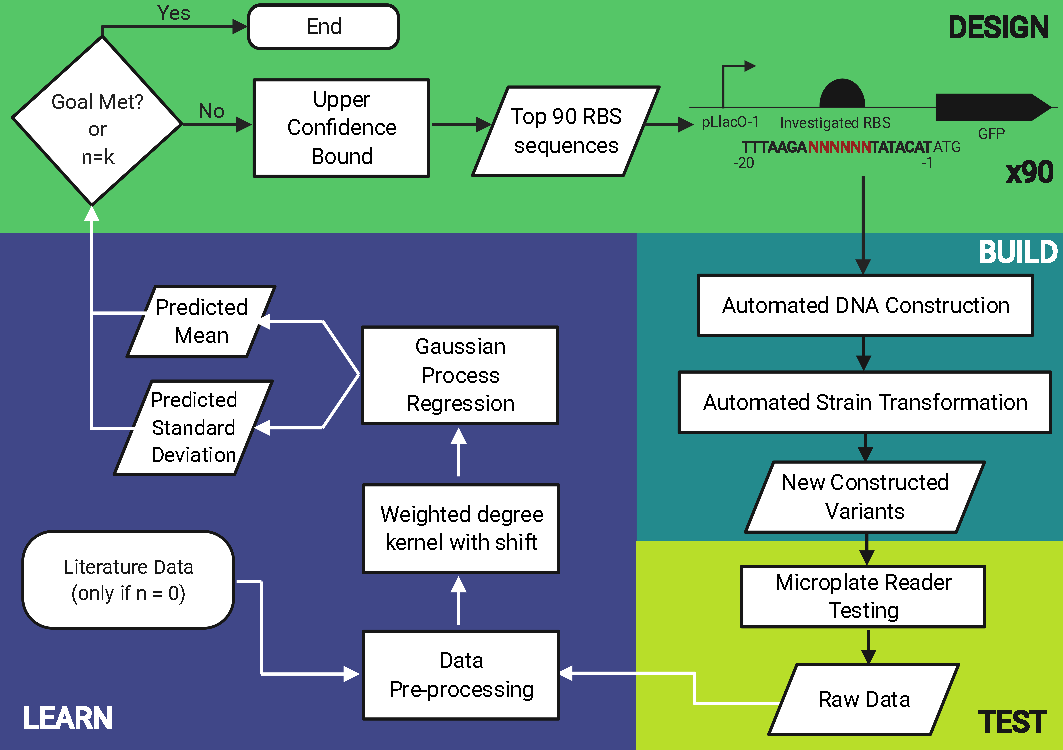
\includegraphics[scale=0.7]{plots/Main_Paper/flowchart.pdf}
    \caption{\textbf{Flowchart of machine learning based experimental design.} The RBS design is recommended by the Upper Confidence Bound Bandit algorithm. After generating the recommendations the RBS are built and tested using automated laboratory methods allowing for rapid construction and testing at scale. Finally, the obtained results are fed back to the prediction algorithm in the learn phase. }
    \label{fig: Flowchart}
\end{figure}

To help us obtain reliable and reproducible results we have employed automation-heavy workflow in the BUILD and TEST phases.
This way we were able to eliminate a big part of sample-to-sample variation as well as human-introduced variation.
Additionally, performing all the procedures directly in 96-well microplate format enabled us to significantly cut down the time required to prepare our variants.\\
In short, the genetic variations of the RBS were introduced to the plasmids with combination of PCR and isothermal assembly. 
The plasmids were then transformed and the resulting transformants were tested using microplate reader.
Vast majority of reactions were prepared using liquid handling equipment.
Similarly, colony picking was done by an automated colony picker.\\

\subsection{Design of the investigated genetic device}

In our genetic design, the investigated RBS controls expression of the Green Fluorescent Protein (GFP) in its mut3b variant. 
By controlling expression of a fluorescent protein with the RBS we can quickly assess the perceived relative TIR by measuring fluorescence of cells harbouring plasmid with the device over time.
Finally, the mRNA is transcribed from an IPTG-inducible promoter pLlacO-1. 
By making the whole device inducible we can synchronise the start of the expression of the GFP in all the cultures by inducing them at the same time with addition of IPTG.

In \emph{E. coli}, the RBS is usually located in the 20 bases upstream of the start codon. 
Additionally, there is a consensus RBS core sequence called the \textit{Shine-Dalgarno sequence}, which in \emph{E. coli} is \textbf{AGGAGG}. 
Here, we put that 20 bp long sequence into focus with main emphasis being put on the 6bp core region
(see detail in Figure \ref{fig: Flowchart}).

Our template RBS sequence, is 20 bps long with the sequence TTTAAGA\textbf{AGGAGA}TATACA.
This sequence is a known to have high TIR and comes with the pBb series plasmids \cite{Lee2011}. 
% Due to poor testing methods that were used for TIR previously we can't claim "highest" cause we don't know how do we compare exactly
Since this is the sequence against which new RBS sequenced will be benchmarked,
we will refer to this sequence as the \textit{benchmark sequence} from now on.
In our design we focus on randomising of the core at positions -8 to -13 (relative to the start codon of the GFP) nucleotides of the RBS and fix others to be the same as the benchmark sequence, i.e. TTTAAGA + NNNNNN + TATACAT, where N can be any choices of A, C, G, T. 
The total experimental (variant) space is then $4^6$ = 4096.
We have experimentally confirmed that changing the core sequence is statistically more impactful on TIR than changes made outside of it (see Supplementary materials).

\subsection{Performance of the recommendation algorithm}
 
The design recommendations were made using the Multi-armed Bandit algorithm.
In short, this algorithm is a stochastic method of probing of the experimental space. 
This algorithm aims at maximising the reward (output) from testing a limited number of instances from a big pool which cannot be wholly tested due to limited resources (time, computational power, capital). 
In our case we use the Upper Confidence Bound version of the algorithm, which focuses its recommendations on sequences that should give highest TIR based on the probabilities computed by the prediction algorithm (see below). 
Another feature of the bandits algorithm is that it balances two parts: the exploration of the unknown (untested) parts of the design space where high TIR RBS can be hidden, and exploitation which goal is querying areas which are known to give relatively high TIRs.
One thing of note is that the bandit algorithm is stochastic, that is it exploits the probabilities of a given event occurring (in this case RBS having a specific TIR). 
As such, it pairs naturally with our prediction algorithm, the Gaussian Process Regression, which provides probability based function regression.

\begin{figure}[!ht]
    \centering
    \begin{subfigure}[b]{0.48\textwidth}
        \centering
        \caption{}
        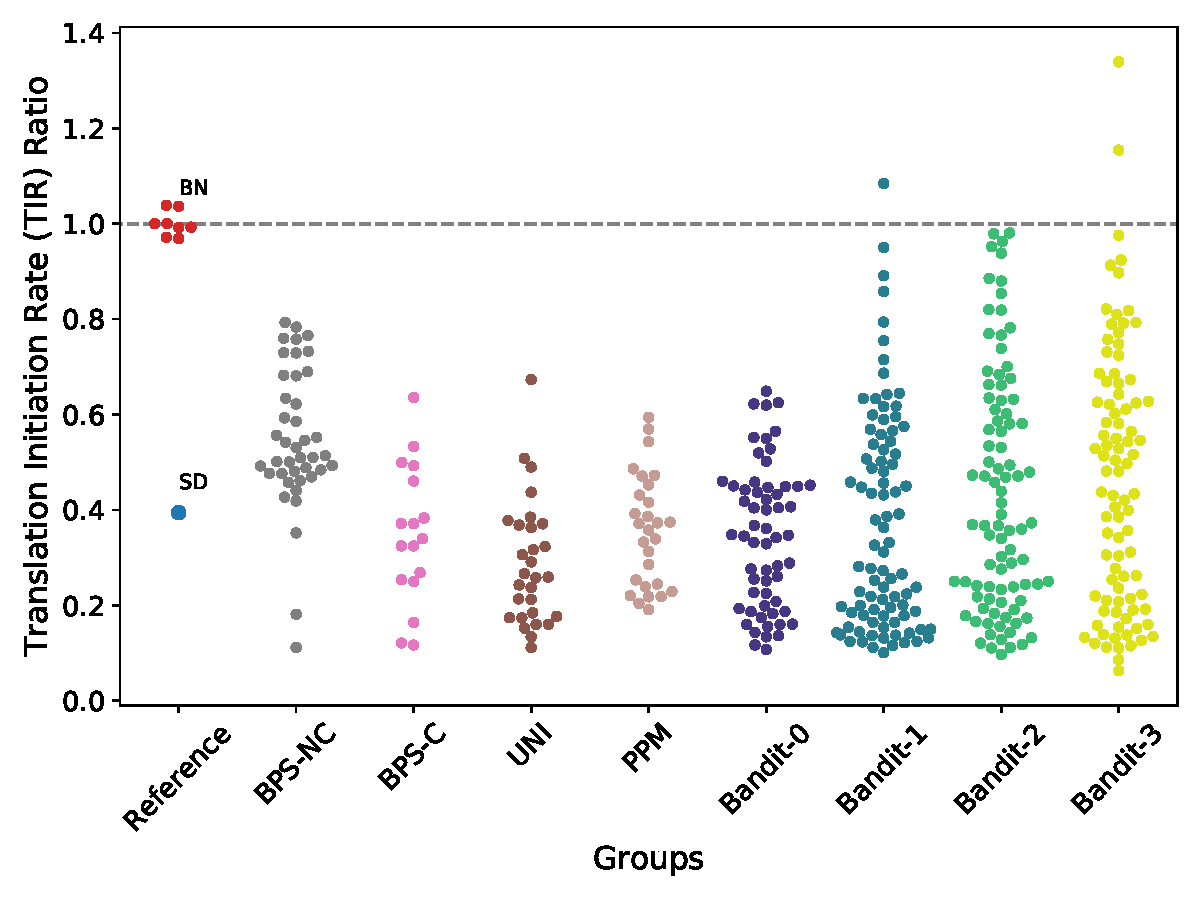
\includegraphics[scale=0.35]{plots/Main_Paper/swarmplot.pdf}
    \end{subfigure}
    % \hfill
    \begin{subfigure}[b]{0.25\textwidth}
        \centering
        \caption{}
        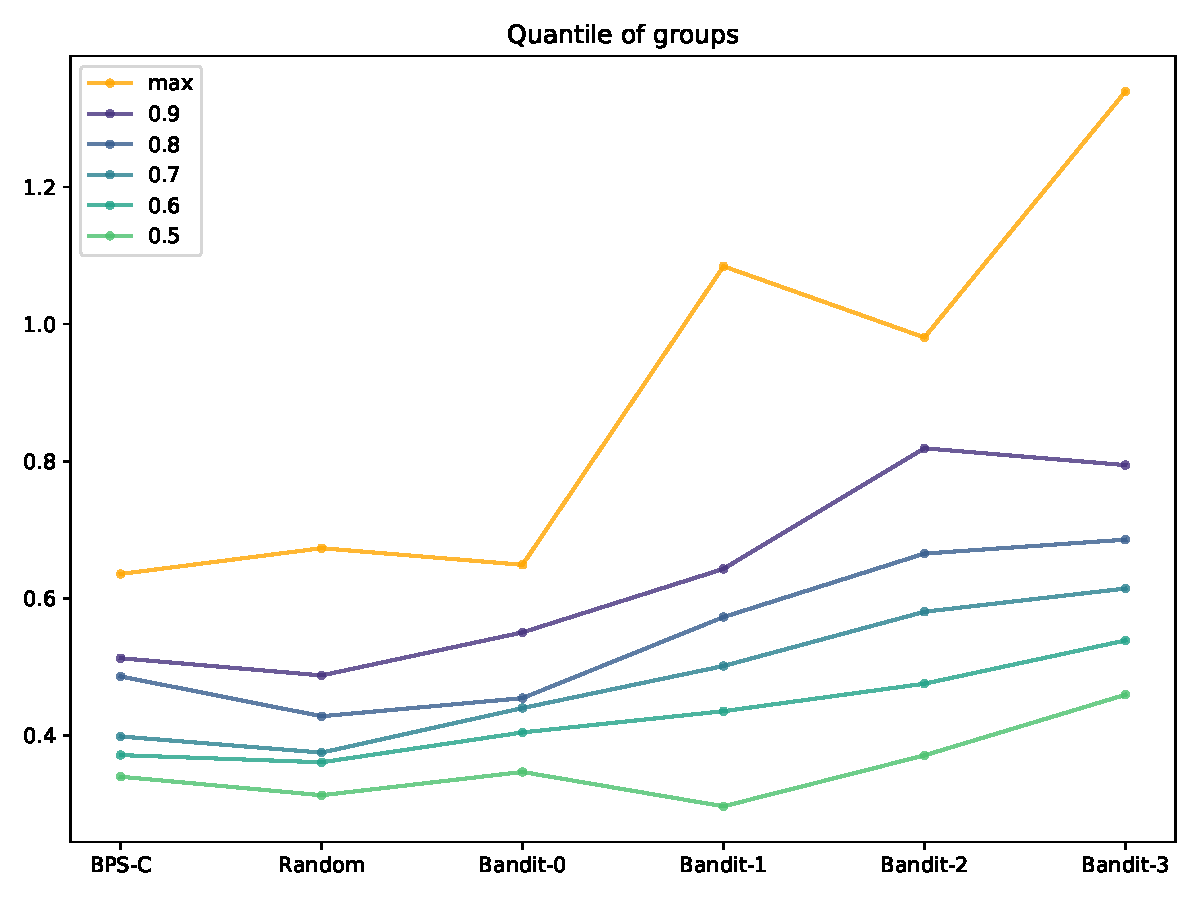
\includegraphics[scale=0.35]{plots/Main_Paper/quantplot.pdf}
    \end{subfigure}
    % \hfill
    \begin{subfigure}[b]{0.25\textwidth}
        \centering
        \caption{}
        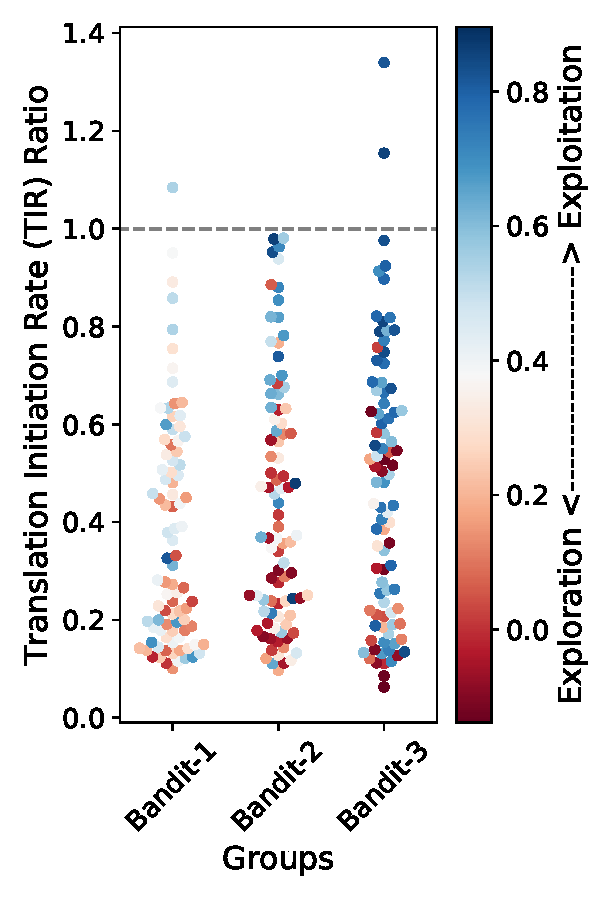
\includegraphics[scale=0.35]{plots/Main_Paper/swarmplot_proj.pdf}
    \end{subfigure}
    \begin{subfigure}[b]{0.48\textwidth}
        \centering
        \caption{}
        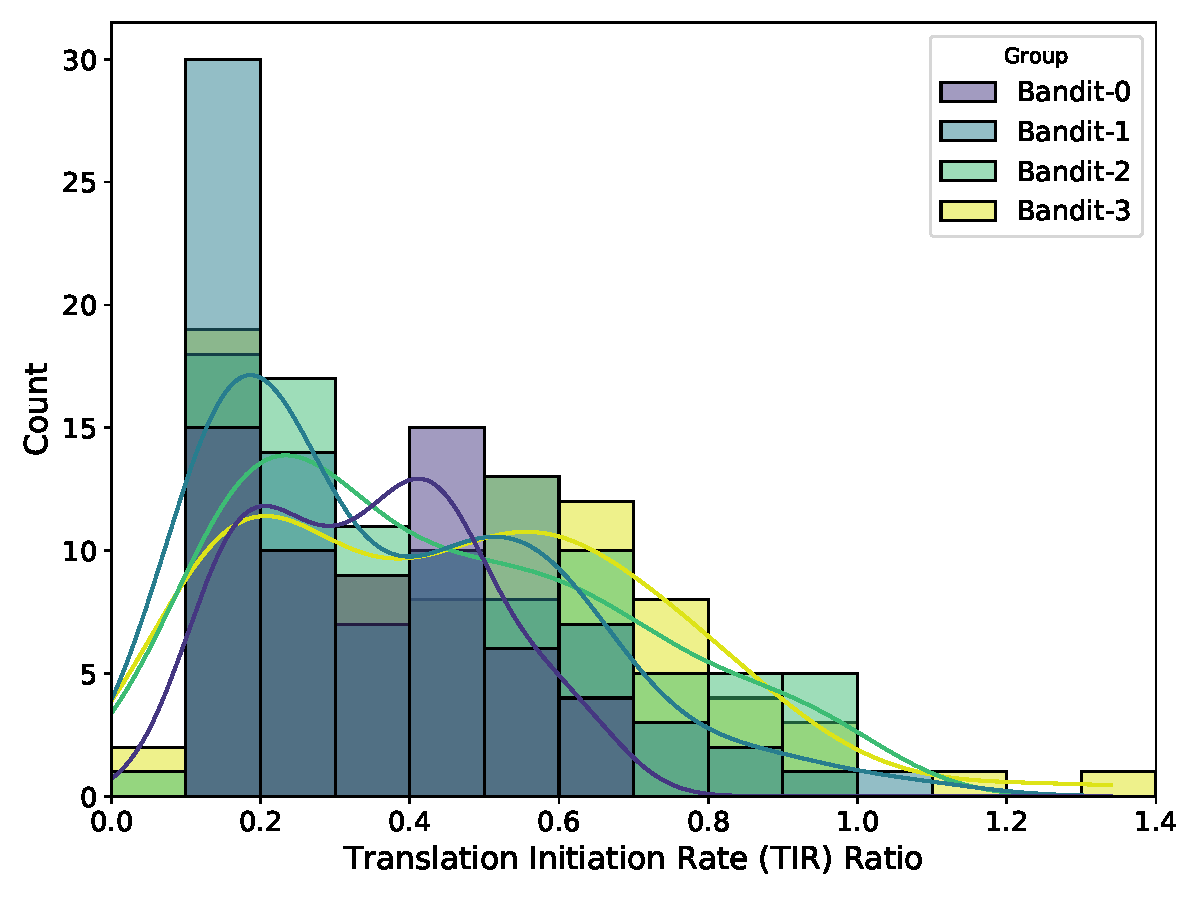
\includegraphics[scale=0.4]{plots/Main_Paper/histogram.pdf}
    \end{subfigure}
    \begin{subfigure}[b]{0.48\textwidth}
        \centering
        \caption{}
        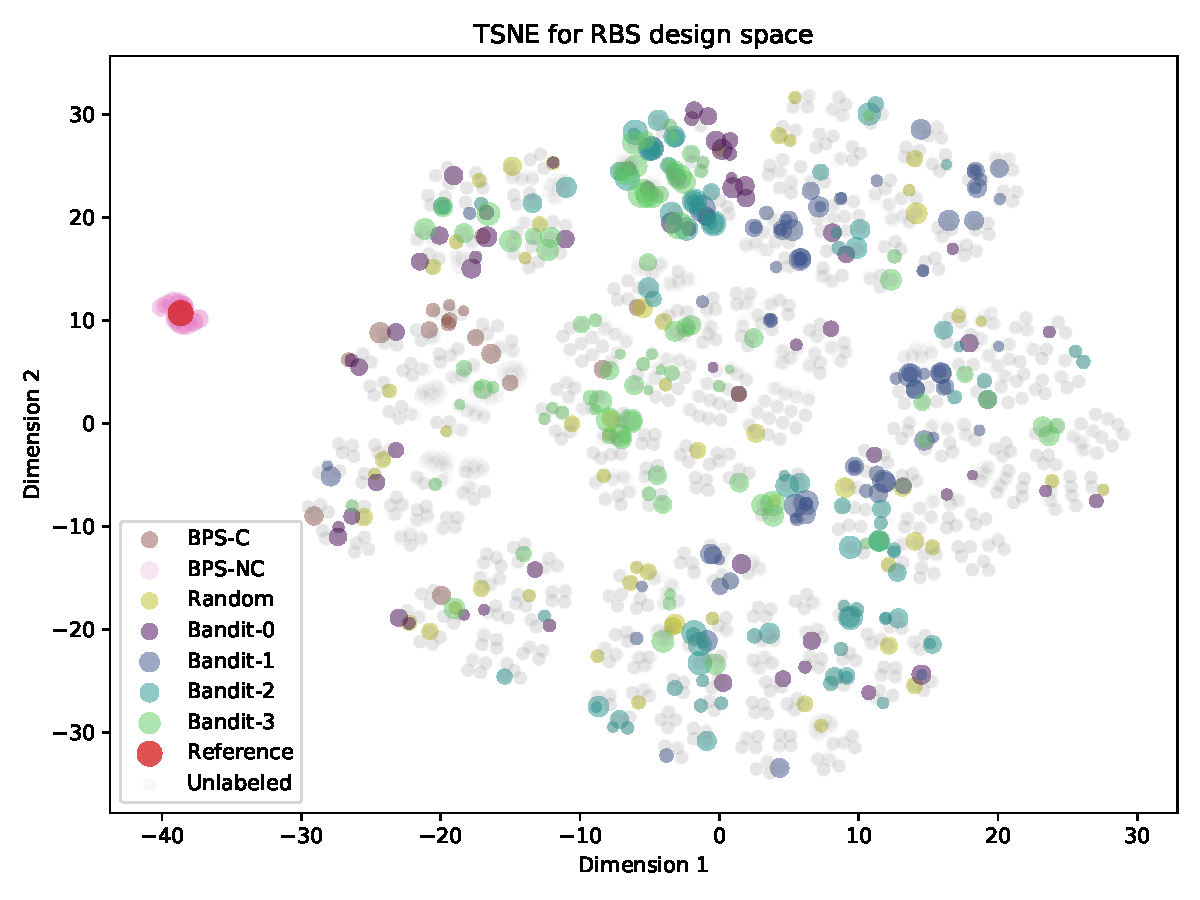
\includegraphics[scale=0.42]{plots/Main_Paper/tsneplot.pdf}
    \end{subfigure}
    % 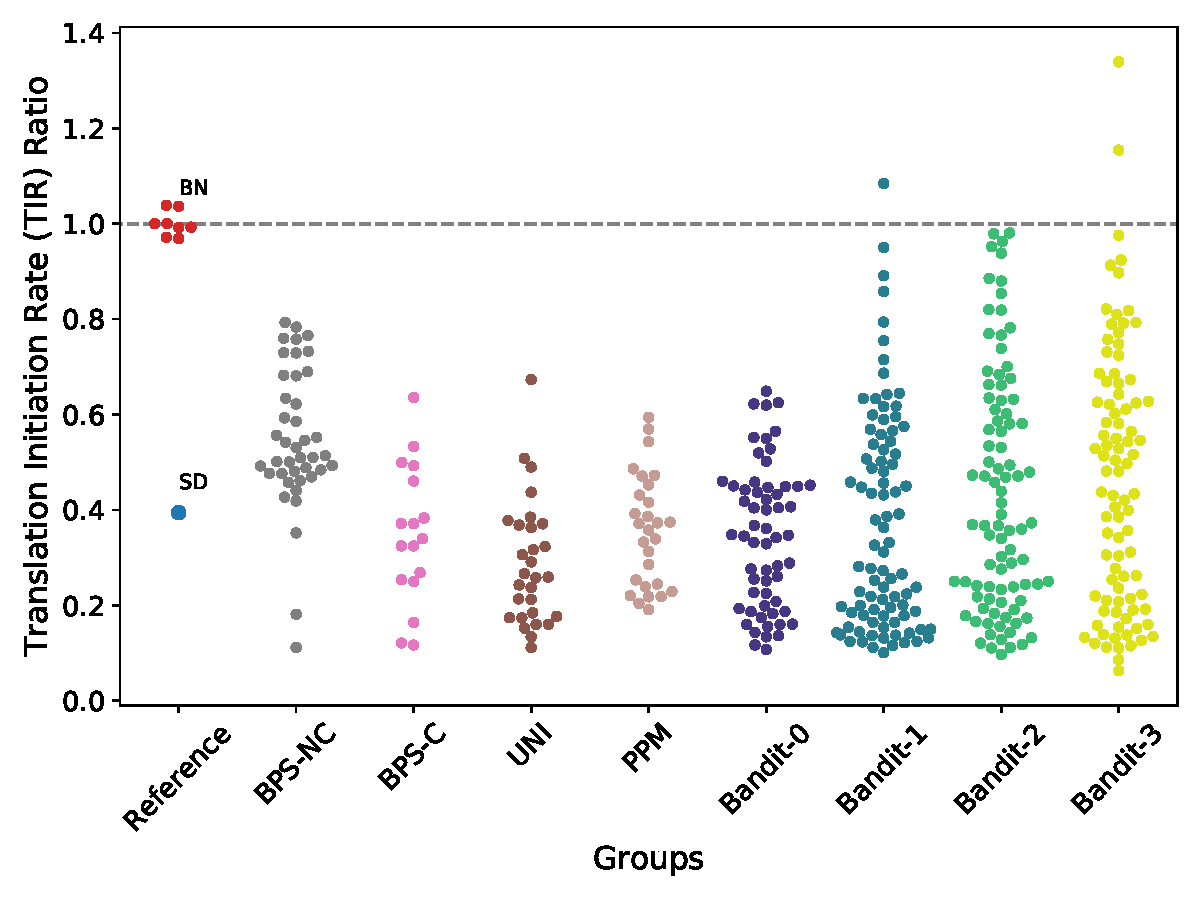
\includegraphics[scale=0.3]{plots/Main_Paper/swarmplot.pdf}
    % 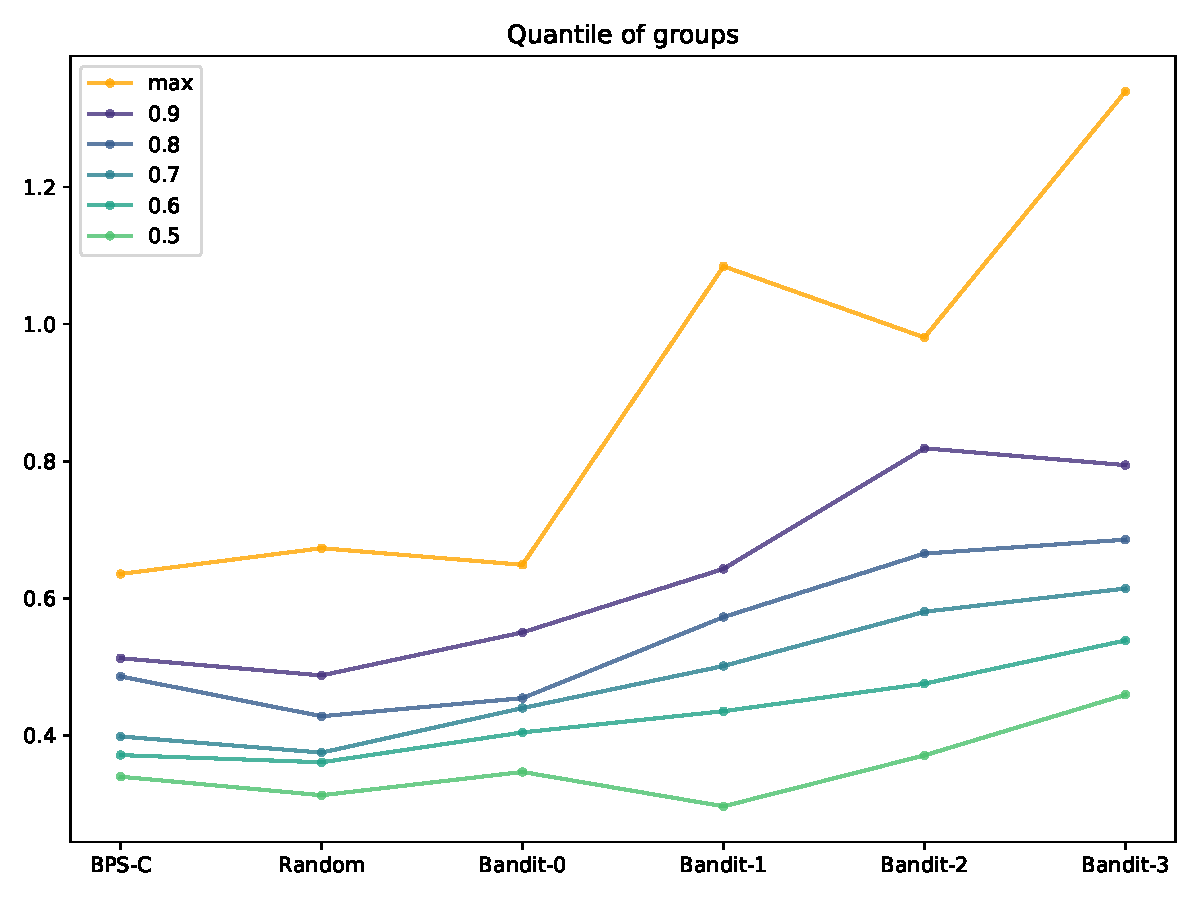
\includegraphics[scale=0.3]{plots/Main_Paper/quantplot.pdf}
    % 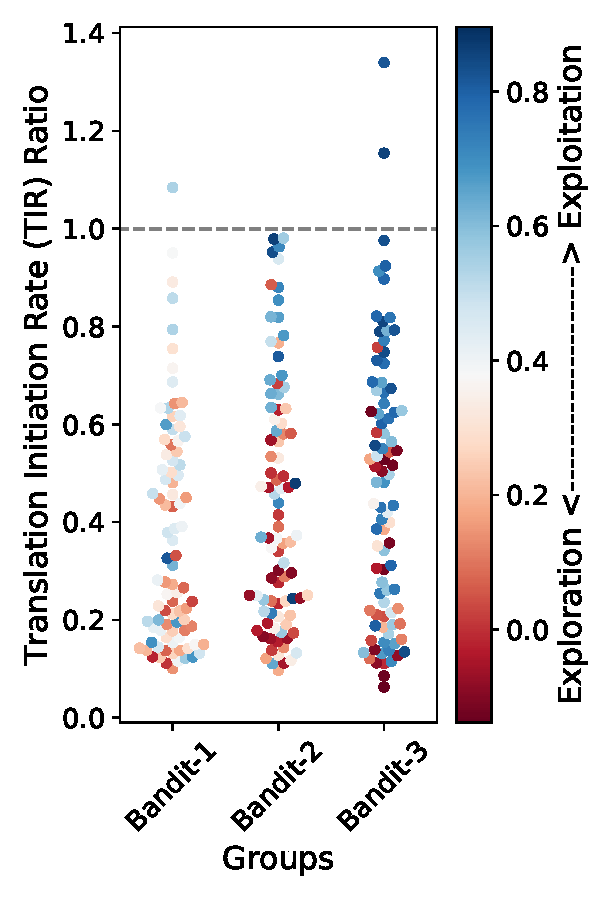
\includegraphics[scale=0.3]{plots/Main_Paper/swarmplot_proj.pdf}
    % 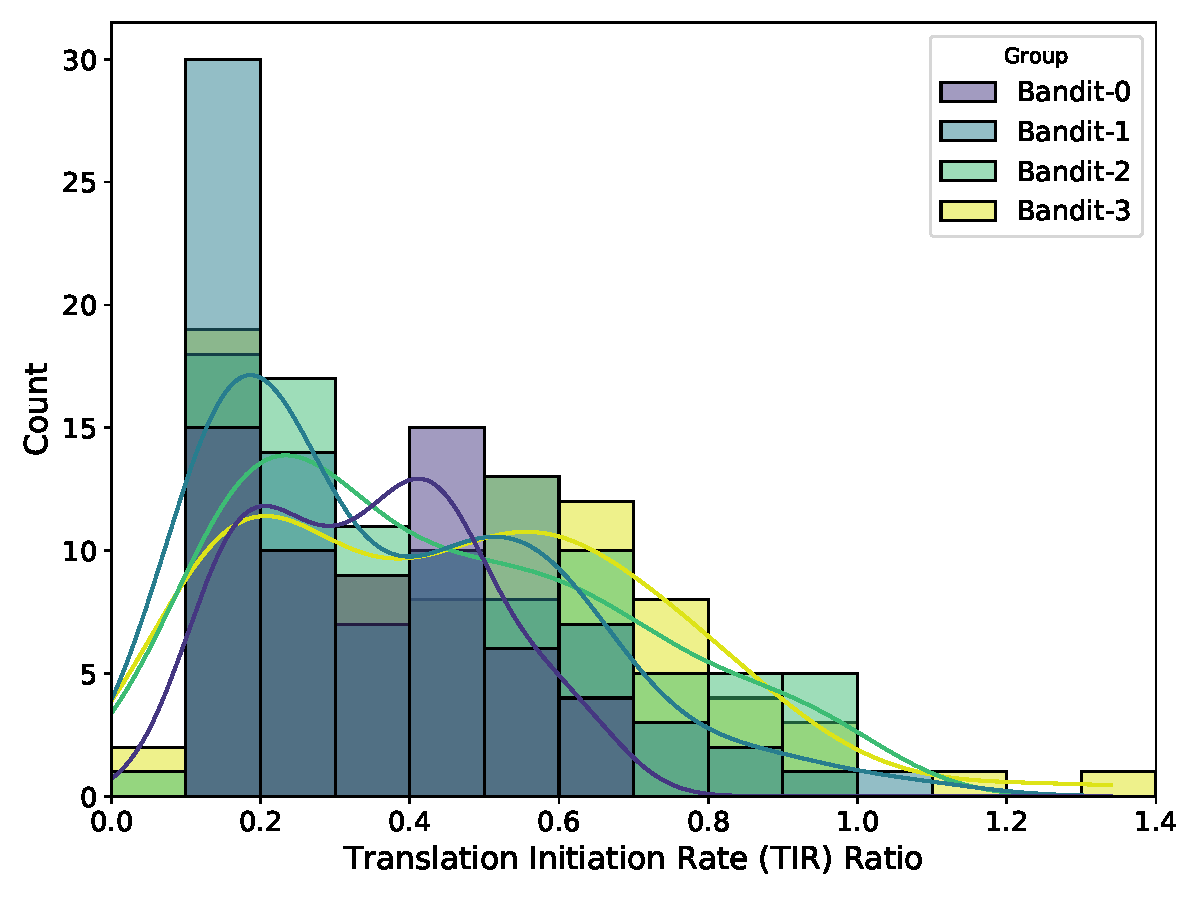
\includegraphics[scale=0.3]{plots/Main_Paper/histogram.pdf}
    % 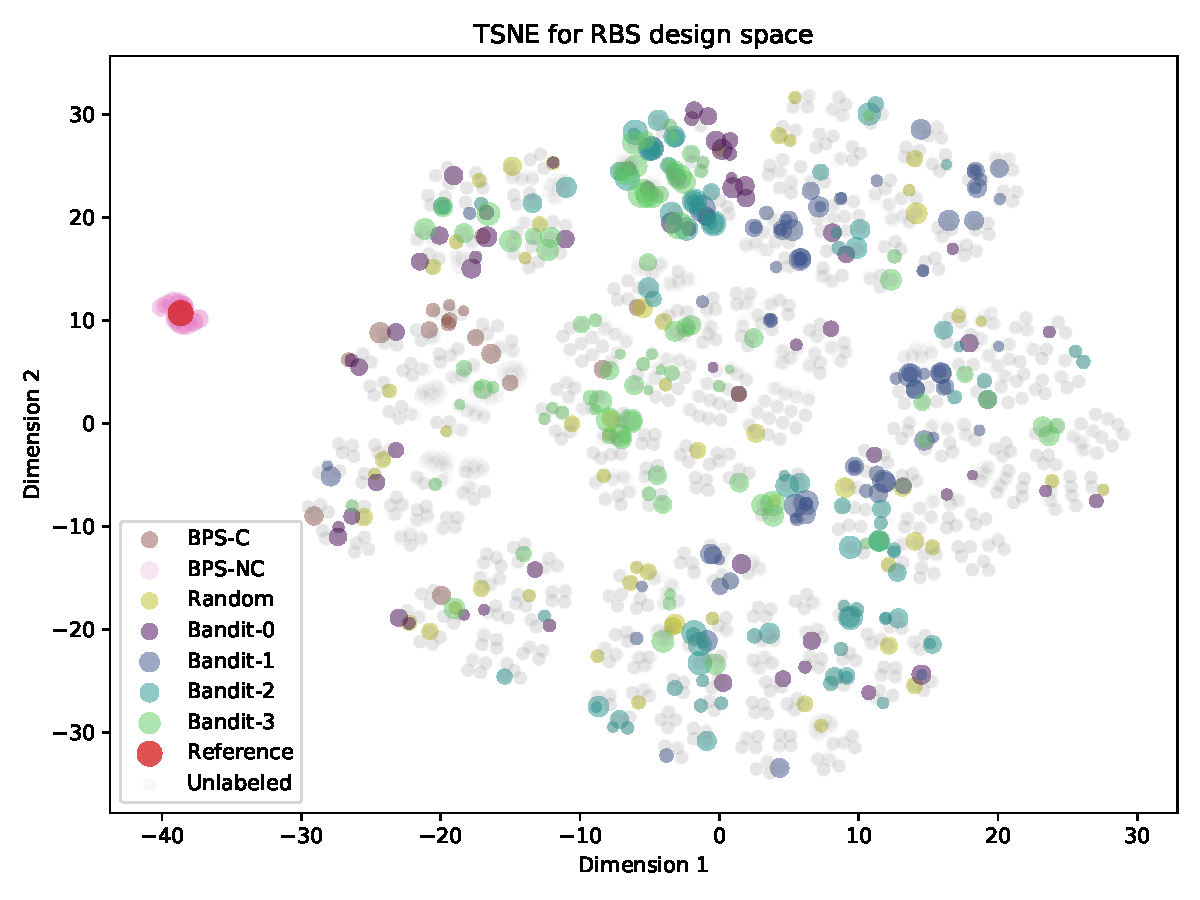
\includegraphics[scale=0.4]{plots/Main_Paper/tsneplot.pdf}
    \caption{
    \textbf{TIRs of RBS groups examined in this study.} 
    The TIR results in all subplots are shown normalised to the respective benchmark sequence sample which acts as internal standard, that is TIR of a given RBS is divided by TIR of the benchmark RBS run in the same plate. 
    \textbf{A)} Swarm plot showing the obtained TIRs divided into RBS groups.
    BPS-NC: base-by-base changes in the non-core region. 
    BPS-C: base-by-base changes in the core region. 
    UNI: Randomly generated sequences with uniform distribution. 
    PPM: Randomly generated sequences with distribution following the PPM for all natural RBS in \emph{E. coli}. 
    Bandit-0/1/2/3 - Bandit algorithm generated results for Round 0, 1, 2 and 3 respectively.
    SD - Shine-Dalgarno sequence.
    Dash line is set to 1 and represents the averaged benchmark sequence TIR for that group. 
    BN - benchmark sequences for all plates. 
    They are not all exactly 1 due to them being shown as separate samples rather than averages.
    \textbf{B)} Line plot showing TIR obtained in a given quantile of results divided into groups as in A).
    % save the random groups which were shown together due to similar distributions.
    UNI and PPM are merged into Random group and BPS-NC was removed due to changes being made outside the core in this group. 
    \textbf{C)} Exploitation v.s. Exploration for Bandit 1-3. Blue-hued points represent exploitation, those hued red represent exploration. 
    \textbf{D)} Histogram with kernel density estimations (KDE) showing distributions of TIRs for Bandit groups.
    \textbf{E)} tSNE plot showing the relative distances between sequences in our design spaces as calculated by our kernel function (weighted degree kernel with shift). 
    The area of the circle represents the experimentally obtained TIR for measured groups.}
    \label{fig: Swarmplot and Quantplot}
\end{figure}

To generate the dataset that the algorithm could learn from we have decided to characterise a total of 450 RBS variants, which constitutes a little over 10\% of the whole experimental space. 
To fit into our automated workflow, we have divided the 450 variants into batches of 90.
In the zeroth round we have tested two batches of designs, for total of 180 variants split as below: 
\begin{itemize}
    \item BPS-NC and BPS-C group: 60 RBS sequences which are subsequent single nucleotide variations of all 20 nucleotides of the original, consensus sequence. This batch is designed to show us influence of such single nucleotide changes on the overall performance of the RBS and the potential impact of changes made beyond the core part (Figure \ref{fig:core_vs_noncore}).
    % \mengyan{put it in main paper?}
    \item UNI group: 30 RBS sequences that were  uniformly randomised, i.e. equal probability of choosing any nucleotide for each position. 
    \item PPM group: 30 RBS sequences randomised based on the position probability matrix (PPM) generated from all the naturally occurring RBS sequences in \emph{E. coli} genome \cite{Stormo1982}.
    \item Bandit-0: 60 RBS sequences recommended by our implementation of recommendation algorithm based on a data set obtained from literature \cite{jervis2018machine}, which contains 113 non-repeated records for 56 unique RBS sequences with the respective TIR.
    This data set has been used due to perceived similarity of its goal to the one of this work - prediction of TIR based on phenotypic output.
\end{itemize}
In the subsequent 3 rounds, all 90 designs were generated using our machine learning algorithm based on the data obtained from the previous rounds (these groups are called Bandit 1 to 3 respectively).

Figure \ref{fig: Swarmplot and Quantplot}A shows the results for all the examined groups. 
% Different randomly generated groups were run together with Bandit 0 (based on literature data) group in Round 0.
% Subsequently, the following rounds from 1 to 3 consisted of only Bandit recommended designs.
In each round, we measure the TIR of benchmark RBS as the internal standard. 
We then obtain the normalised TIR (called \textit{TIR ratio}) by taking the ratio between the raw TIR and the average TIR of benchmark sequences in each round (which are run in triplicate in each round).
All Round 0 groups (BPS-NC, BPS-C, UNI, PPM, Bandit-0) have performed worse than our benchmark sequence in terms of TIR. 
The Bandit-0 group performed poorly, despite being machine learning driven, due to being trained on literature data.
However, starting from Round 1, where the bandit algorithm was fed data from the Round 0 the results become much better, with a number of sequences that perform better than the consensus Shine-Dalgarno sequence and in one case better than the benchmark (by 8\%).
In round 2 we have observed further improvement by getting more sequences that showed TIR on levels similar to our benchmark sequence.
Finally, in round 3 the algorithm identified two sequences that were 34\% and 15\% stronger than the benchmark sequence.
Figure \ref{fig: Swarmplot and Quantplot}B shows the same results but divided into quantiles where the specific point for a given group is showing the highest TIR for that quantile.
The gradual increase for all quantiles can be observed for all Bandit groups suggesting algorithms' better understanding of the experimental space with more data.
The decreased result in the 0.9th qunatile compared to the max value for Bandit 3 group can be attributed to the increased emphasis on exploitation that has been set for the that round compared to others.
We see that effect in Figure \ref{fig: Swarmplot and Quantplot} c), where we coloured the data points for Bandit 1-3 groups according to their relative exploration - exploitation affinity.
We can see the RBSs with high TIRs (blue, with high predicted mean) tend to come from exploitation the design space whereas the explorative points (red, with high predicted standard deviation) give relatively low TIR but expand our knowledge about the unknown part of the design space. 
Figure \ref{fig: Swarmplot and Quantplot}D shows the TIRs of RBSs tested in the Bandit groups divided into bins of width of 0.1 TIR ratio.
KDE plots have been overlaid to depict the calculated density for each group.
The increase of prevalence of later bandit groups in the higher bins is evident, especially for Bandit 2 and 3 constituting the bulk of results in the $>0.8$ TIR ratio bins.
\mengyan{do we want to address two-mode pattern (due to the exploration and exploitation.)}
\maciej{I did that in a later section.}
\mengyan{I recommend to mention the observation and point to where you discuss it.}
In \ref{fig: Swarmplot and Quantplot}E we show a tSNE plot depicting the experimental space.
Each RBS is located on the plot according to its distance to other RBSs as calculated by our kernel function.
We can see the RBSs recommended by Bandit groups have covered majority of the design space. 
A number of clusters were targeted by our recommendation algorithm.
For example, the circled clusters labelled as "G-Rich Clusters" have been actively recommended by the algorithm.
More specifically, sequences with more or equal to 4 guanines in any position constituted 10\% of the randomly selected sequences and 5, 9, 16 and finally 25\% in each of the 4 Bandit guided batches respectively.

\subsection{Prediction of RBS performance}

Our recommendation algorithm selects new designs based on means and uncertainties calculated by our prediction algorithm.
This algorithm creates a model which takes the RBS sequences as input and predicts the TIR values with uncertainty level about the prediction, based on the experimental data.
For this study, we have used the Gaussian Process regression (GPR) as our prediction method.
GPR is a Bayesian approach and has been widely used for experimental design \cite{srinivas2012information, romero_navigating_2013}.
% Such a stochastic prediction method fits biological processes naturally, since they are highly stochastic as well. 
The explicit representation of model uncertainty provides further guide for efficient searching through large experimental space of possible sequences.\\
A crucial ingredient in a Gaussian Process predictor \cite{Rasmussen2004} is the kernel (covariance) function, which captures the similarity between data points, in our case RBS sequences.
Specifically, kernel function implicitly embeds RBS sequences into high-dimensional feature space which makes the regression process easier.
For Bandit designs in Round 0, since we only had access to limited number of data points from literature, we chose to use one of the basic string kernels, the \textit{spectrum kernel} \cite{leslie2001spectrum} to process the core 6bp and dot product kernel \cite{Rasmussen2004} (with one-hot embedding) to process the 7bp flanking sequences both upstream and downstream of the core sequence.
For subsequent rounds, we used 
% a more powerful \maciej{more powerful in what sense?} kernel function, 
the \textit{weighted degree kernel with shift} (WDS) \cite{ratsch_rase_2005_wds}, which has been shown to have good performance in various prediction tasks \cite{Ben-Hur2008}.
The WDS not only counts the matches of substrings of a certain length (i.e. kmers), but also takes into account the positional information and shifting of substrings.
For example, two sequences A\textbf{CCTGA} and \textbf{CCTGA}A are in 1-shift.
The relative distances between sequences calculated by our kernel function are shown in figure \ref{fig: Swarmplot and Quantplot}E.\\

Figure \ref{fig: Scatterplot} shows how our algorithm performed in terms of predictions in each round. 
As expected, the predictions in Round 0 were poor due to use of approximated data. 
The predictions improved for the subsequent rounds, from R\textsuperscript{2} of 0.065 for round 0 to R\textsuperscript{2} of 0.27 for round 3.
Similarly, the Spearman correlation coefficient rose from 0.27 for Round 0 to 0.48 for Round 3.
% Interestingly there wasn't much difference in fitness parameters between Round 1-3.
% One interesting point is that despite relatively low correlations between predicted and true values our recommendation algorithm performed very well.
One important point to note is that the predictions are also influenced by our recommendation choices. 
In each round, we select a number of data points for exploration, which means that these data points, when tested, have a high chance of having real mean different to what was predicted.
However, this is still very useful information for future predictions as it allows us to understand the underlying space better.
    
\begin{figure}[!ht]
    \centering
    \begin{subfigure}[b]{0.49\textwidth}
        \centering
        \caption{}
        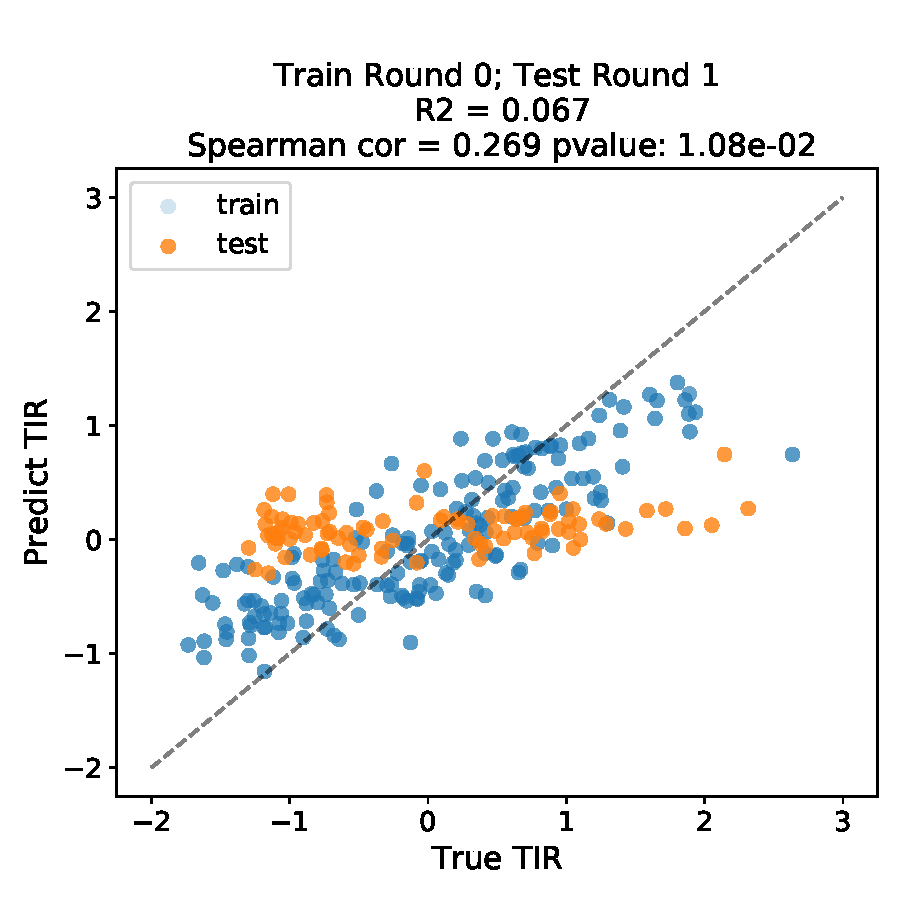
\includegraphics[scale=0.4]{plots/Main_Paper/scatter_abc1_FF_0.pdf}
    \end{subfigure}
    % \hfill
    \begin{subfigure}[b]{0.49\textwidth}
        \centering
        \caption{}
        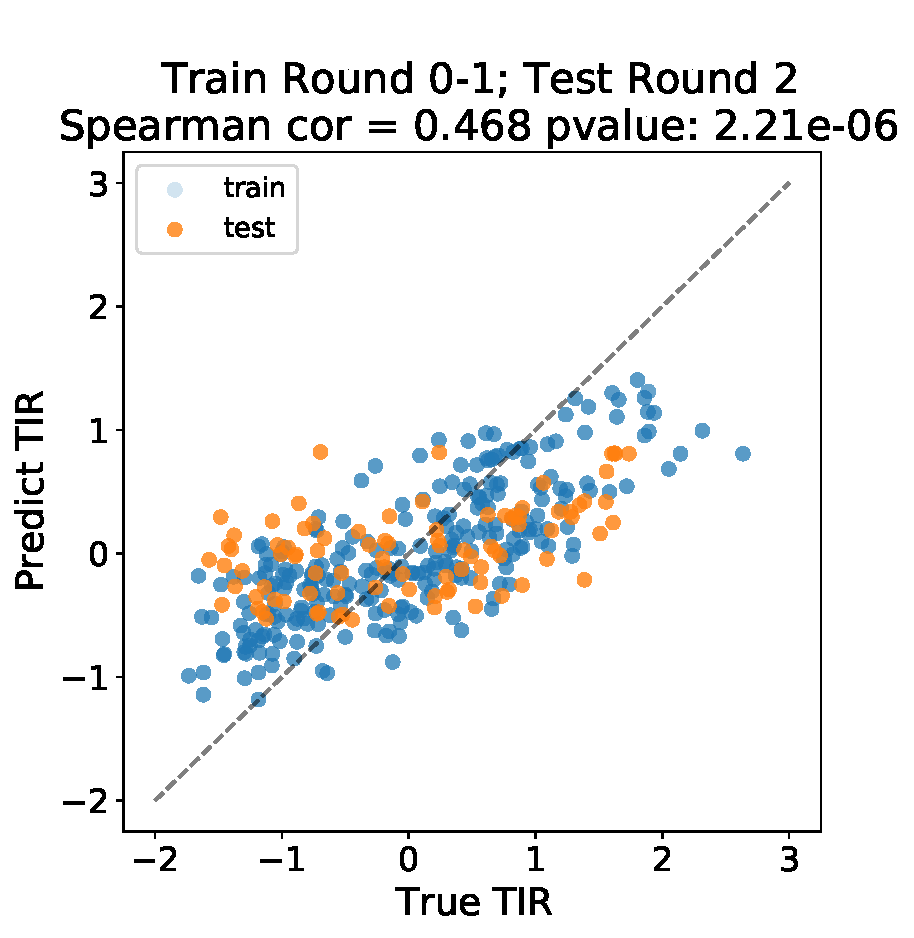
\includegraphics[scale=0.4]{plots/Main_Paper/scatter_abc1_FF_1.pdf}
    \end{subfigure}
    % \hfill
    \begin{subfigure}[b]{0.49\textwidth}
        \centering
        \caption{}
        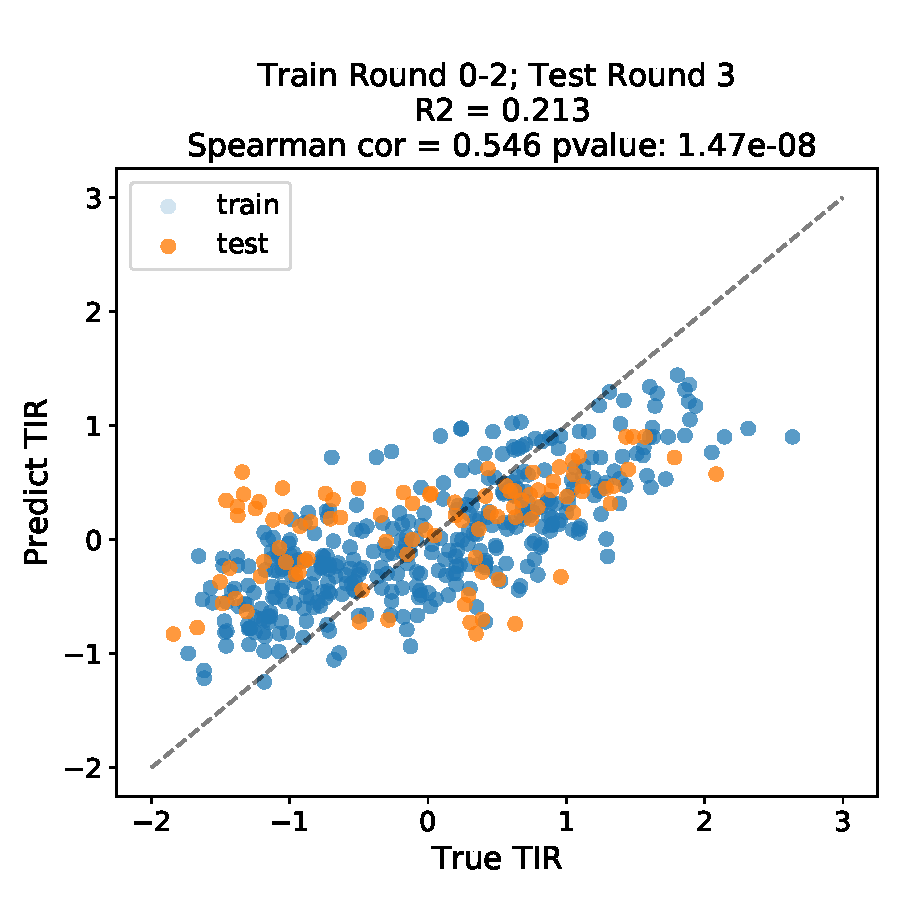
\includegraphics[scale=0.4]{plots/Main_Paper/scatter_abc1_FF_2.pdf}
    \end{subfigure}
    \begin{subfigure}[b]{0.49\textwidth}
        \centering
        \caption{}
        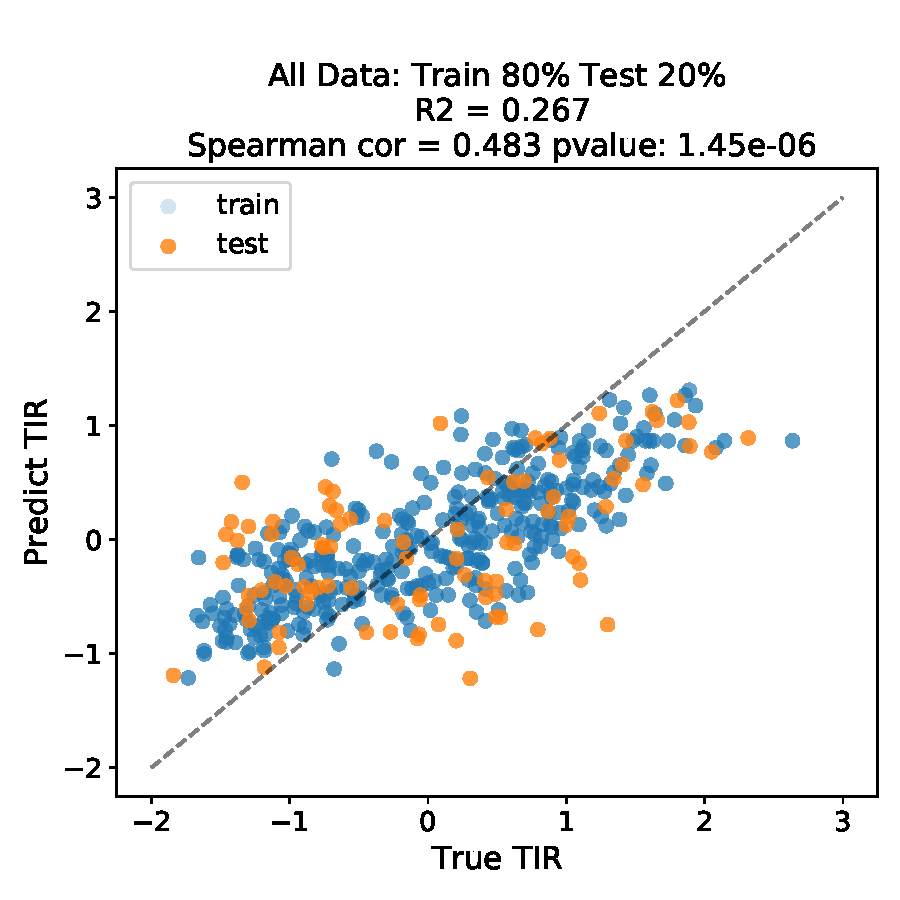
\includegraphics[scale=0.4]{plots/Main_Paper/scatter_abc1_FF_3.pdf}
    \end{subfigure}
    \caption{\textbf{Predictions generalise to held out data.} The scatter plots A-D are showing the performance of our prediction algorithm (GPR with WDS kernel, with maximum k-mer as 6 and maximum shift as 1) calculated after each of the rounds.
    Note the TIR values are normalised TIR based on the standardisation described in section \ref{sec: method data pre-procesing}, which is different from the TIR ratio reported in the Figure \ref{fig: Swarmplot and Quantplot}.
    The values of 
    $R^2$ and Spearman correlation coefficient (with corresponding p-value) are all provided for each plot.
    The p-value decreases with round increases, which shows increasing strong evidence about the Spearman correlation between our prediction and measured TIR. 
    }
    \label{fig: Scatterplot}
\end{figure}

\subsection{Characteristics of the tested sequences}

Figure \ref{fig:Library characteristics}A shows the sequence logo calculated for the Top 30 (in terms of TIR ration) of our sequences.
It is generally understood that guanine rich sequences are promoting strong transcription.
This expected bias towards guanine is clearly visible for all positions in our Top 30 RBSs.
This result combined with the Bandits' algorithm bias towards the G rich cluster shown in figure \ref{fig: Swarmplot and Quantplot}D reinforces the notion that our algorithm successfully identified G rich sequences as ones with high TIR probability.

\begin{figure}[!t]
     \centering
     \begin{subfigure}[b]{0.49\textwidth}
         \centering
         \caption{}
         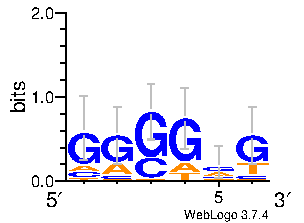
\includegraphics[scale=1.2]{plots/Main_Paper/TOP30_logo.pdf}
     \end{subfigure}
     \hfill
     \begin{subfigure}[b]{0.49\textwidth}
         \centering
         \caption{}
         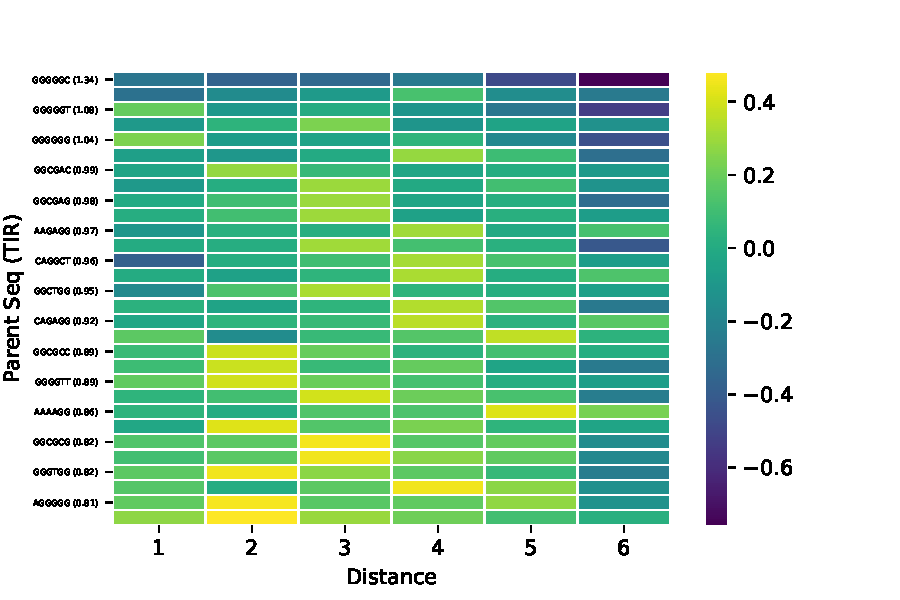
\includegraphics[scale=0.5]{plots/Main_Paper/Hd_Heatmap.pdf}
     \end{subfigure}
     \caption{\textbf{Characteristics of strong RBSs.} A) Sequence logo calculated for the Top 30 tested sequences. B) Heatmap showing what edit (Hamming) distance is required for positive change in TIR for RBS with high and medium TIR. The temperature scale shows the difference between a given RBS on y axis and the RBS with strongest TIR at the given distance. Every second RBS is labelled for increased legibility. }
     \label{fig:Library characteristics}
\end{figure}

\begin{table}[!h]
\centering
\begin{minipage}[c]{0.6\textwidth}
\centering
\begin{tabular}{|c|c|}
\hline
\textbf{Characteristics of the library}                                                       & \textbf{Statistics} \\ \hline
Total experimental space                                                                      & 4096                \\ \hline
Planned constructs                                                                            & 450                 \\ \hline
Successfully constructed                                                                      & 445                 \\ \hline
Sequences with CV\textless{}40\%                                                              & 79\%                \\ \hline
Sequences with CV\textless{}20\%                                                              & 27\%                \\ \hline
\begin{tabular}[c]{@{}c@{}}Efficiency of bandit design \\ (compared with random)\end{tabular} & 2                   \\ \hline
Raw TIR range                                                                                     &      [4.9258, 105.377]               \\ \hline
TIR ratio range                                                                                     &      [0.0626, 1.3393]               \\ \hline
\end{tabular}
\end{minipage}
\begin{minipage}[c]{0.38\textwidth}
\centering
% Please add the following required packages to your document preamble:
% \usepackage[table,xcdraw]{xcolor}
% If you use beamer only pass "xcolor=table" option, i.e. \documentclass[xcolor=table]{beamer}
\begin{tabular}{|c|c|}
\hline
\textbf{Top RBS Core} & \textbf{TIR Ratio} \\ \hline
GGGGGC                & 1.3393             \\ \hline
GGGGGT                & 1.1544             \\ \hline
GGCTAT                & 1.084              \\ \hline
\textbf{AGGAGA}                & 1                  \\ \hline
GGCGTT                & 0.9805             \\ \hline
GGGGGG                & 0.9788             \\ \hline
GGCGAC                & 0.9758             \\ \hline
CAGGAG                & 0.9629             \\ \hline
GGCGAG                & 0.9519             \\ \hline
\textbf{AGGAGG}                & 0.3941             \\ \hline
\end{tabular}
\end{minipage}
\caption{Characteristics of the library. \mengyan{write caption here}
For Efficiency of bandit design:
random = {set of TIR that are in UNI and PPM};
bandit = {set of TIR that are in bandit 0,1,2,3}.
The ratio of the max bandit to the max random: $1.34/0.67$ = 2;
The ratio of the 0.9 quantile bandit to the 0.9 quantile random: $0.82/0.49$ = 1.67.}
\end{table}

Another interesting characteristic uncovered by our research is the perceived editing distance between two sequences required for  improvement in the TIR when the given RBS' TIR is already high. 
We define the editing distance as Hamming distance, that is, how many positions have to be changed to get from one sequence to the other (Hamming distance of 0 means that the sequences are identical and 6 means that they are two completely different sequences).
Figure \ref{fig:Library characteristics}B shows what edit distance is required for positive change in TIR for RBS with TIR $>0.75$.
For RBS with high TIR ($>1$), the minimum distance that is required for increase of TIR is 2, with edit distance between 2 and 5 giving similar results.
For RBS with medium TIR ($<1$), a distance of 1 is enough to produce a meaningful increase in TIR.
That means that as the TIR of examined RBSs increases, exploring sequences which are more dissimilar to the current candidates tends to give meaningful improvement. 
The low rate of natural mutations will be very slow to explore more dissimilar sequences on such a short distance \cite{Lee2012},
which indicate that Adaptive Laboratory Evolution may not be able to find very strong RBSs within limited budget.  
In other words, because the examined sequence is relatively short (6bp in a wider 20bp context) the time to accumulate 2 or more changes in the RBS region required for meaningful increase in TIR might be prohibitively long.
In such cases, a directed process should be strongly encouraged.
This is in line with common practices in e.g. protein engineering, where similar approaches, that is making more directed changes, are often observed \cite{Jackel2008}.

Finally, our strong sequences did not show neither strong binding to the anti-sense sequence of the ribosome known to bind to RBS nor any obvious secondary structures that could explain their TIRs (see Supplementary).
This result combined with the unexpectedly bimodal nature of KDEs in Figure \ref{fig: Swarmplot and Quantplot} reinforces the notion based on the previously reported literature \cite{Saito2020,EspahBorujeni2016} that there may be a number of different mechanisms governing the probability of effective RBS-ribosome binding.\\


\section{Discussion}

In this work, we have shown how machine learning and high-throughput, automated laboratory methods can be used to efficiently generate a library of small parts, in this case bacterial RBS. 
We have used Gaussian Process regression to predict the shape of our function and Upper Confidence Bound Bandit algorithm to recommend sequences to be tested.
We have investigated a number of methods of digitising the DNA sequence, finally settling on Weighted Degree Kernel with Shift method, which fit well into our prediction method.
We building and testing, we have performed bulk of our experiments using automation to increase their speed, reliability and reproducibility.
By using our workflow, we have found very strong RBS sequences and we have generated an extensive library of diverse RBS that can be used in the future studies.
We have achieved this despite the relatively low accuracy of our predictions, which means that the presented algorithms are robust and able to identify the right signal in a noisy environment. \\

There are still open questions that need to be addressed for applying machine learning in synthetic biology.
For example, how can we understand the language of RBS sequences better?
In other words, can we extract more biologically important information from the decisions made by our algorithms?
Another example would be - given a small amount of RBS sequences tested, how can machine learning algorithm provide more accurate predictions and uncertainty measurement? 
Finally, another question with high impact on the performance of the workflow is - how should we choose the parameters which controls the exploration-exploitation rate? \\

We have found our approach bringing machine learning and synthetic biology experts very powerful.
We envision to that the pairing of machine learning with high-throughput automation will keep delivering a high number of good quality datasets nad improved methods for biological engineering.\\

In the future, we hope to extend the algorithm to other, more complicated genetic elements.
This could include, for example, promoters and terminators.
However, its important to note that the complexity of the task quickly increases with the length of the sequence.
This is because the experimental space grows exponentially with the number of examined positions and so the space becomes increasingly hard to cover with experiments.
To solve this problem, a different algorithms or experimental techniques might be needed, but the general workflow can be reused.\\

\mengyan{We should try to alter the discussion in terms of our three-sentence story, along with open questions (in a more positive way) and future work.}

\section{Methods}

\subsection{Plasmid Design}

We have used the pBbB6c-GFP plasmid for all our designs. This plasmid comes with GFP mut3b CDS inducible with addition of IPTG. The original RBS for the GFP CDS was replaced with combination of PCR and isothermal assembly. Primers and the assembly strategy have been generated using the Teselagen DESIGN software (Teselagen Biotechnology).

\subsection{PCR}
PCR amplification of the cloning inserts was done using Q5 High-Fidelity 2X Master Mix (NEB, catalogue no. M0492L). 20 \(\mu\)L reactions were prepared by dispensing each of the 10 \(\mu\)M reverse primers into a well of a 96-well PCR plate using the Labcyte Echo Liquid Handler. A mastermix consisting of polymerase premix, plasmid DNA template, and the single 10 forward primer was prepared by and dispensed by hand. Reactions were run using Touchdown PCR or standard PCR cycling methods in BioRad C1000 thermal cyclers. Then, samples were incubated at 37$^{\circ}$C for 60 minutes, followed by a 20-minute heat inactivation step at 80$^{\circ}$C.
Capillary electrophoresis of PCR products was performed using the Agilent Technologies ZAG DNA Analyzer system. 2\(\mu\)L of each PCR reaction was electrophoresed using the ZAG 130 dsDNA Kit (75-20000bp) or ZAG 110 dsDNA Kit (35-5000bp) (Agilent Technologies, catalogue no. ZAG-110-5000; ZAG-130-5000). ProSize Data Analysis Software (Agilent Technologies) was used to generated gel images from the sample chromatograms and sizes were estimated by reference to the upper and lower DNA markers spiked into each sample and a DNA ladder run in well H12 of each sample plate. 

\subsection{Isothermal DNA Assembly}
Constructs were assembled using NEBuilder HiFi DNA Assembly Master Mix (NEB, catalogue no. E2621L). Samples were incubated at 37$^{\circ}$C for 60 minutes, followed by a 20-minute heat inactivation step at 80$^{\circ}$C. Reactions consisting of the common fragment and the variable fragment were prepared using the Echo acoustic liquid handler, to a final volume of 5 or 10\(\mu\)L . Assemblies were run in the thermal cycler for 1 hour at 50$^{\circ}$C, followed by an infinite hold step at 4$^{\circ}$C.

\subsection{\textit{E. coli} transformation}
The DH5α cell line (Thermo Fisher Scientific, catalogue no. 18265017) was made chemically competent using the Mix & Go \textit{E. coli} Transformation Kit & Buffer Set (Zymo Research, catalogue no. T3001). 20\(\mu\)L of cells was aliquoted into each well of a cold 96-well PCR plate and stored at -80$^{\circ}$C for later use. Plates of cells were thawed on a -20$^{\circ}$C cold block before 3µL of the assembly product was added and mixed using the CyBio FeliX liquid handler. Cells were incubated on a cold block for 2-5 minutes before being plated in a 96 square grid on Omnitrays containing LB (BD, catalogue no. ***) with 34\(\mu\)g/mL chloramphenicol (Sigma, catalogue no. ***). Multiple dilutions of cells in LB were prepared and plated in parallel on Omnitrays in 96 square grid. Plates were incubated overnight at 37$^{\circ}$C.

\subsection{Automated colony picking and culturing}
A Singer Instruments PIXL colony picker was used to select individual colonies from the transformation plates. Each selected colony was used to inoculate 1mL of selective medium in a 2mL square well 96 plate. They were then cultured overnight in 37$^{\circ}$C with shaking (~300rpm).

\subsection{Glycerol stock preparation}
100\(\mu\)L of sterile 80\% (v/v) glycerol and 100\(\mu\)L of overnight culture were combined in the wells of a 96 deep (2mL) round well plate using the CyBio Felix liquid handler. They were then sealed with a 96-well silicon sealing mat and transferred to a -80$^{\circ}$C freezer. 

\subsection{Cuture analysis}
Overnight cultures were started by inoculating 1mL of LB medium supplemented with 34\(\mu\)g/mL chloramphenicol with ~2\(\mu\)L of the glycerol stock in a 96 deep (2mL) round well plate. Cultures were incubated at 37$^{\circ}$C with shaking (~300rpm) for ~17 hours. The following morning, 20\(\mu\)L of overnight culture was added to 980\(\mu\)L of fresh selection medium and precultures were grown at 37$^{\circ}$C with shaking in 2mL round well 96 plate. 
After 90 minutes, two parallel cultures were prepared in flat-bottom clear polystyrene 96-well plates and were induced with 500\(\mu\)M IPTG – one plate of 300\(\mu\)L cultures for flow cytometry analysis (induced with 1.5\(\mu\)L of 0.1M IPTG) and one plate of 200\(\mu\)L cultures for plate reader analysis (induced with 1.0\(\mu\)L of 0.1M IPTG).
•	Cytation 5 acquisition and incubation/shaking settings
•	CytoFLEX S acquisition settings

\subsection{Machine learning experimental design}

To automatically design the RBS sequences in batch using machine learning, we consider two parts: 
1) Design an regression algorithm which takes the RBS sequences as input and returns the predicted TIR scores and the confidence intervals. 
2) Design an online learning approach which recommends the RBS sequences based on the predicted TIR scores and confidence intervals. 
Such online learning approach provides the $\textit{exploitation-exploration balance}$ that we use to control our machine learning process.

With the goal of finding RBS sequences with the largest possible TIR score after a total number of rounds $N$,  we consider our experimental design problem as sequentially optimising an unknown reward function $f: \mathcal{D} \rightarrow \mathbb{R}$, where $\mathcal{D}$ is the set containing all RBS sequence points, and $f(\mathbf{x})$ is the TIR score at $\mathbf{x}$. 
In each round $t$, we choose a set of $m$ points $\mathcal{S}_t \subset \mathcal{D}$ and observe the function values of each points in the selected set $\mathcal{S}_t$, i.e. $y_i = f(\mathbf{x}_i) + \epsilon_i$, for all $i \in \mathcal{S}$, where $\epsilon_i$ is the noise (we assume the noise is following Gaussian distribution with unknown mean and variance). This noise is influenced by the accuracy of the RBS predictor and other experimental interference (e.g. time, temperature, operator, etc.). 

For regression model, we consider the \textit{Gaussian Process Regression (GPR)}.
A Gaussian process regression model \cite{Rasmussen2004} is a Bayesian approach which provides uncertainty measurements on predictions. 
We model $f$ as a sample from a \textit{Gaussian process} $\mathcal{G} \mathcal{P}(\mu(\mathbf{x}), k(\mathbf{x}, \mathbf{x'}))$, which is specified by the mean function $\mu(\mathbf{x})=\mathbb{E}[f(\mathbf{x})]$ and the kernel (or covariance) function $k\left(\mathbf{x}, \mathbf{x}^{\prime}\right)=\mathbb{E}[(f(\mathbf{x})-\left.\mu(\mathbf{x}))\left(f\left(\mathbf{x}^{\prime}\right)-\mu\left(\mathbf{x}^{\prime}\right)\right)\right]$.
Denote the training testing data as $X, X_{*}$, and the training label as $\mathbf{y}$.
Then the posterior of the test points (i.e. predictive distributions) is given by the conditional distribution $\mathbf{f}_\ast | X, \mathbf{y}, X_\ast \sim \mathcal{N}(\bar{\mathbf{f}}_\ast, cov(\mathbf{f}_\ast))$, where
\begin{align}
\overline{\mathbf{f}}_{*} & \triangleq \mathbb{E}\left[\mathbf{f}_{*} \mid X, \mathbf{y}, X_{*}\right]=K\left(X_{*}, X\right)\left[K(X, X)+\alpha^{2} I\right]^{-1} \mathbf{y} \\
\label{Eq: predicted variance in main paper}
\operatorname{cov}\left(\mathbf{f}_{*}\right) &=K\left(X_{*}, X_{*}\right)-K\left(X_{*}, X\right)\left[K(X, X)+\alpha^{2} I\right]^{-1} K\left(X, X_{*}\right) 
\end{align}
%For noisy test targets $\mathbf{y}_\ast$, we can compute the predictive distribution by adding $\alpha^2 I$ to the variance term $cov(\mathbf{f}_\ast)$ in Eq. (\ref{Eq: predicted variance in main paper}).

To represent the RBS sequences and formulate the similarity between sequences, we use the \textit{weighted degree kernel with shift} \cite{ratsch_rase_2005} to specify the kernel function of $GP$.  
The weighted degree kernel with shift extends the spectrum kernel \cite{leslie2001spectrum, ben2008support} 
by considering the positional information and allowing some positional shifts of matching substrings.
The spectrum kernel and the weighted degree kernel with shifts are string kernels, which take two sequences as inputs and outputs a scalar value which represents the similarities between the two sequences. 
We define spectrum kernel firstly,
\begin{align}
        k_\ell^{\text{Spec}}(\textbf{x}, \textbf{x}^\prime) =\left\langle\phi_{\ell}^{\mathrm{Spec}}(\mathbf{x}), \phi_{\ell}^{\mathrm{Spec}}\left(\mathbf{x}^{\prime}\right)\right\rangle = \phi_{\ell}^{\mathrm{Spec}}(\mathbf{x})^T \phi_{\ell}^{\mathrm{Spec}}\left(\mathbf{x}^{\prime}\right).
    \end{align}
 where $\mathbf{x}, \mathbf{x}^\prime$ are two RBS sequences in $\mathcal{D}$ over an alphabet $\Sigma$. We denote the number of letters in the alphabet as $|\Sigma|$. 
$\phi_{\ell}^{\mathrm{spec}}(\mathbf{x})$ maps the sequence $\textbf{x}$ into a $|\Sigma|^\ell$ dimensional feature space, where each dimension is the count of the number of one of the $|\Sigma|^\ell$ possible strings $s$ of length $\ell$. 
Let $X, X^\prime$ be two metrics which include $n$ sequences, and $\Phi_d^{Spec}(X) \in \mathbb{R}^{n \times |\Sigma|^{\ell}}$, then the spectrum kernel over metrics is 
    \begin{align}
         K_\ell^{\text{Spec}}(X, X^\prime) = \Phi_{\ell}^{\mathrm{Spec}}(X) \Phi_{\ell}^{\mathrm{Spec}}\left(X^{\prime}\right)^T.
    \end{align}
The weighted degree kernel with shift is defined upon the spectrum kernel, with flexibility of adjusting the substring length $d$, the start position $l$ and the shift length $s$. WDS kernel counts the match of kmers at corresponding positions in two sequences as shown in the following,
\begin{align}
        k_\ell^{WDS}(\mathbf{x}, \mathbf{x}^\prime) 
        &= \sum_{d=1}^{\ell} \beta_d \sum_{l=1}^{L-d+1} \gamma_l \sum_{s = 0, s + l \leq L}^{S(l)} \delta_s
        \left(k_d^{Spec}(\mathbf{x}_{[l+s:l+s+d]}, \mathbf{x}_{[l:l+d]}^\prime) + (k_d^{Spec}(\mathbf{x}_{[l:l+d]}, \mathbf{x}_{[l+s:l+s+d]}^\prime)\right)\\
        &= \sum_{d=1}^{\ell} \beta_d \sum_{l=1}^{L-d+1} \gamma_l \sum_{s = 0, s + l \leq L}^{S(l)} \delta_s
        \left(\mathbb{I}(\mathbf{x}_{[l+s:l+s+d]} = \mathbf{x}_{[l:l+d]}^\prime) + (\mathbb{I}(\mathbf{x}_{[l:l+d]}= \mathbf{x}_{[l+s:l+s+d]}^\prime)\right),
\end{align}
where $\beta_d = \frac{2(\ell - d + 1)}{\ell(\ell+1)}, \delta_s = \frac{1}{2(s+1)}$, $\gamma_l$ is a weighting over the position in the
sequence, where we choose to use a uniform weighting over the sequences, i.e. $\gamma_l = 1/L$. $S(l)$ determines the shift
range at position $l$. 
%Since the sequences in provided data have the pattern that the core area is different from each other, and other areas are similar. So the kernel for Gaussian Process we are using is the sum of kernels, for core areas we use spectrum kernel with string as input directly, and for other areas we use one-hot encoding and dot product kernel for simplicity.
    
    
%  For recommendations, we consider the \textit{Upper Confidence Bound (UCB)} type algorithms. 
%  As one popular type of the bandit algorithms \cite{lattimore2018bandit}, the UCB type of algorithms are based on the \textit{optimism in the face of uncertainty},
 %provide various approaches to sequential design where an agent adaptively chooses one or more options among several actions based on certain policies. In our work we used the Upper Confidence Bound version of that algorithm, which is based on the \textit{optimism in the face of uncertainty}. The UCB algorithm, as the name suggests,
%  which basically select RBS sequences with the maximum upper confidence bound constructed by the sum of the predicted mean and $n$ standard deviation ($n > 0$), i.e. $\operatorname{argmax}_{\mathbf{x}_i \in \mathcal{D}} \left( \mu_t(\mathbf{x}_i) + \beta_t \sigma_t(\mathbf{x}_i)\right)$,
%     where $\beta_t$ is a hyperparameter balancing the exploitation and exploration, 
%     $\mu_t(\mathbf{x}_i), \sigma_t(\mathbf{x}_i)$ are the predicted mean and standard deviation at round $t$ for the sequence $\mathbf{x}_i$. 

For recommending RBS sequences to label, we consider the Upper Confidence Bound (UCB) algorithm, 
%which is based on the \textit{optimism in the face of uncertainty}, 
selecting RBS sequences with the maximum upper confidence bound at round $t$, i.e.
\begin{align}
\label{Eq: GPUCB}
    \operatorname{argmax}_{\mathbf{x}_i \in \mathcal{D}} \left( \mu_{t-1}(\mathbf{x}_i) + \beta_t \sigma_{t-1}(\mathbf{x}_i)\right),
\end{align}
where $\beta_t$ is a hyperparmeter balancing the exploitation and exploration, 
$\mu_t(\mathbf{x}_i), \sigma_t(\mathbf{x}_i)$ are the predicted mean and standard deviation at round $t$ for the sequence $\mathbf{x}_i$.

Since labelling sequences is time-consuming, it is unrealistic to recommend sequence sequentially (i.e. one-by-one) and waiting for the label for each round.
Therefore we consider recommending sequences in batch and use Gaussian Process Batch Upper Confidence Bound (GP-BUCB) algorithm  \cite{desautels2012parallelizing}.
With batches of size $B$, the feedback mapping is then defined as $fb[t] = \lfloor(t-1) / B\rfloor B$, i.e. 
\begin{align}
    \mathrm{fb}[t]=\left\{\begin{array}{cl}
    0 & : t \in\{1, \ldots, B\} \\
    B & : t \in\{B+1, \ldots, 2 B\} \\
    2 B & : t \in\{2 B+1, \ldots, 3 B\} \\
    & \vdots
    \end{array}\right.
\end{align}


A key property of Gaussian Process regression is that the predictive variance in Eq. (\ref{Eq: predicted variance in main paper}) only depends on observed points (i.e. features), but not on the labels of those observed points. 
So one can compute the posterior variance without actually observing the labels. 
The GP-BUCB policy is to select sequences that
\begin{align}
    \operatorname{argmax}_{\mathbf{x}_i \in \mathcal{D}} \left( \mu_{fb[t]}(\mathbf{x}_i) + \beta_t \sigma_{t-1}(\mathbf{x}_i)\right).
\end{align}
And only update $y_{t^{\prime}}=f\left(\boldsymbol{x}_{t^{\prime}}\right)+\varepsilon_{t^{\prime}} \text { for } t^{\prime} \in\{\mathrm{fb}[t]+1, \ldots, \mathrm{fb}[t+1]\}$ at the end of each batch ($\mathrm{fb}[t]<\mathrm{fb}[t+1]$). 
This is equivalent to sequential GP-UCB with \textit{hallucinated observations} $\boldsymbol{y}_{\mathrm{fb}[t]+1: t-1}=\left[\mu_{\mathrm{fb}[t]}\left(\boldsymbol{x}_{\mathrm{fb}[t]+1}\right), \ldots, \mu_{\mathrm{fb}[t]}\left(\boldsymbol{x}_{t-1}\right)\right]$, while the posterior variance decreases. 


\begin{figure}[t]
    \centering
    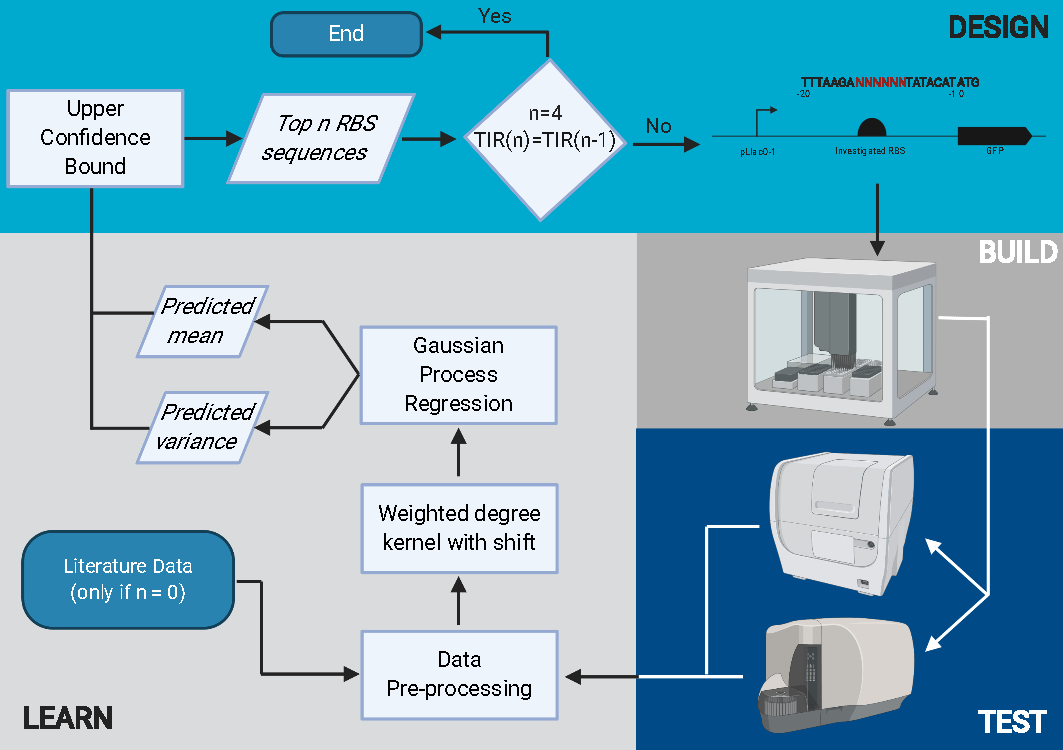
\includegraphics[scale=0.7]{plots/flowchart.pdf}
    \caption{Flowchart of machine learning based experimental design.}
    \label{fig: flowchart of machine learning based experimental design.}
\end{figure}







\section*{Code and data availability}

All code and data required to reproduce the results is available at Github: \url{https://github.com/mholowko/SynbioML}

\section*{Contributions}
Zhang M. and Ong C. S. designed and implemented the machine learning algorithms and workflow. Holowko M. B. and Hayman Zumpe H. have designed and performed the laboratory experiments. Holowko M. B. and Ong C. S. conceived and planned the project. All authors analysed the data, contributed to and reviewed the manuscript.

\section*{Competing interests}
The authors declare no competing interests.

\section*{Acknowledgments}
The authors would like to acknowlege CSIRO's Machine Learning and Artificial Intelligence, and Synthetic Biology Future Science Platforms for providing funding for this research. The authors would also like to thank CSIRO BioFoundry for help with performing the experiments.


\newpage

\printbibliography

\clearpage

\appendix
\textbf{Supplementary}

\section{Extended Machine Learning Discussion}

\subsection{Reproducible Plots}
In this section, we put reproducible plots and will update the plots when we get full results. 

\begin{figure}[h]
    \centering
    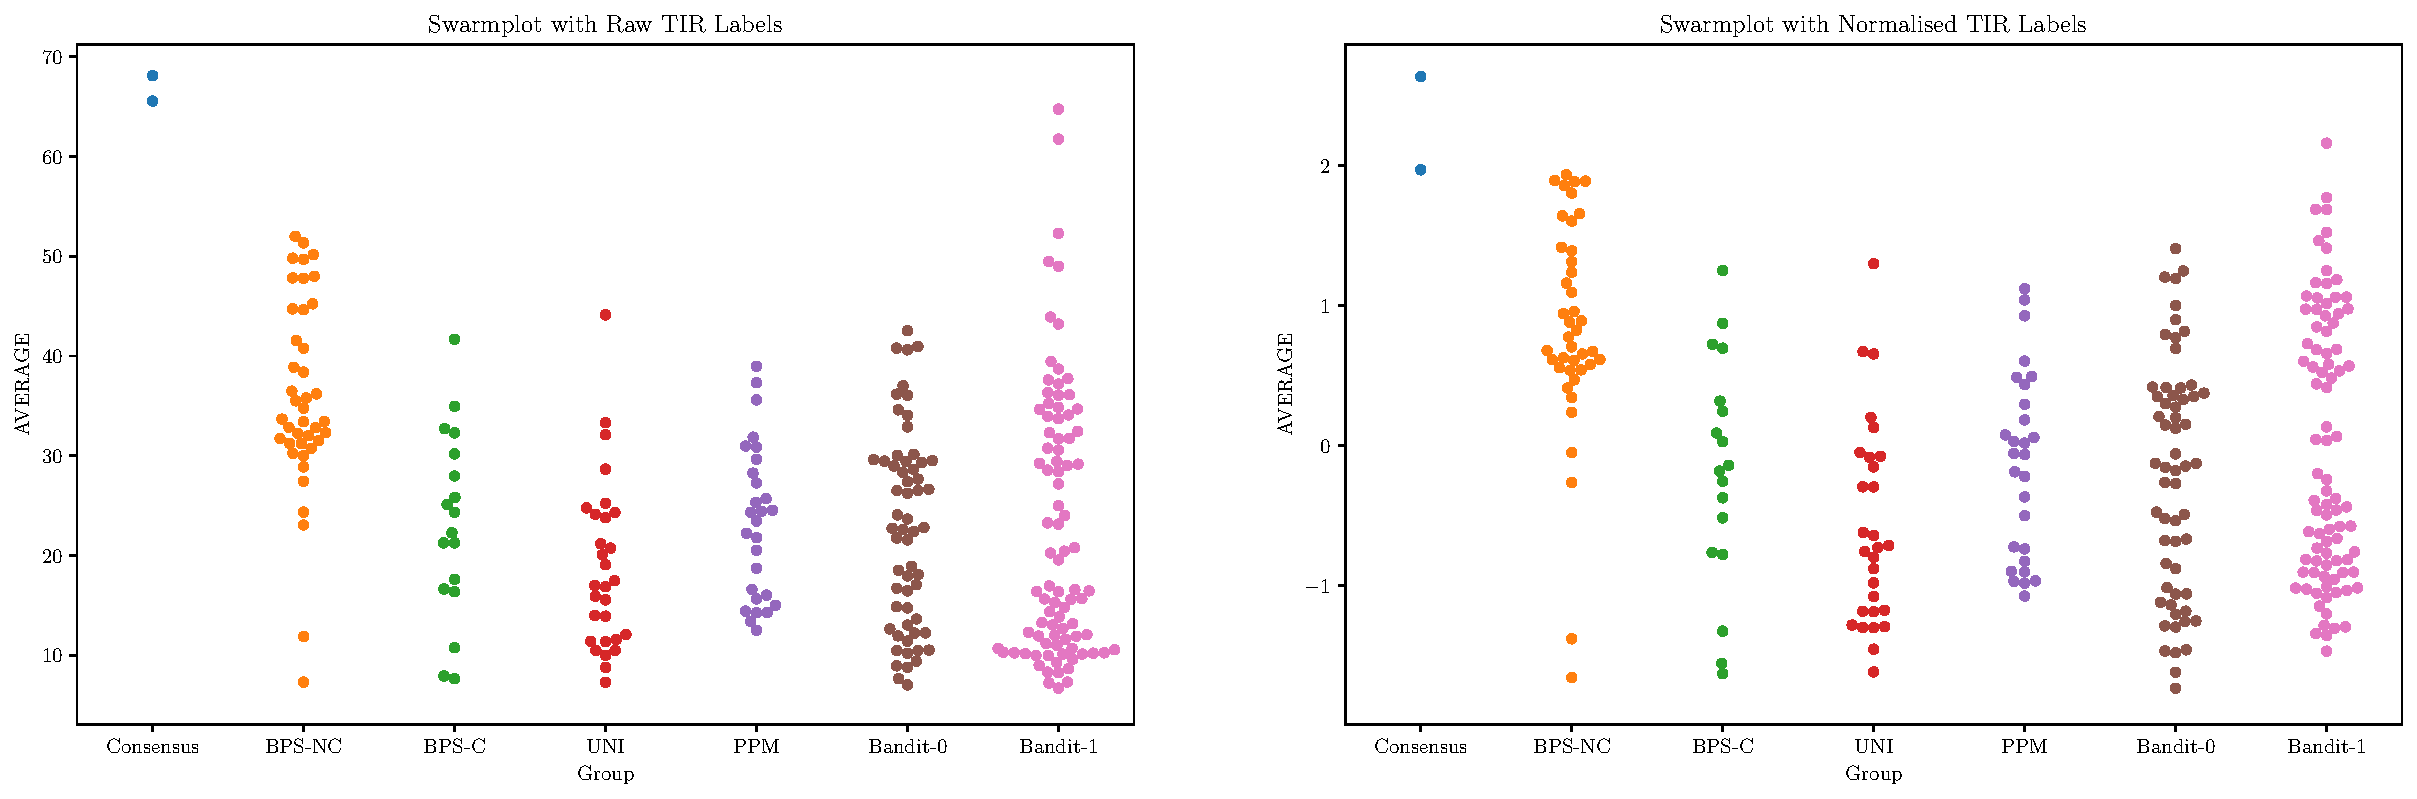
\includegraphics[scale = 0.4]{plots/Supplementary/swarmplots.pdf}
    \caption{Swarmplots for different groups, with raw (left) and normalised (right) TIR labels (averaged over 6 replicates). 
    Group names represent: Consensus (consensus sequence tested in different round); BPS-NC (bps noncore); BPS-C (bps core); UNI (uniformly random); PPM (position-based probability matrix); Bandit-0 (bandit design for round 0); Bandit-1 (bandit design for round 1).}
    \label{fig:swarmplots.}
\end{figure}

\begin{figure}
    \centering
    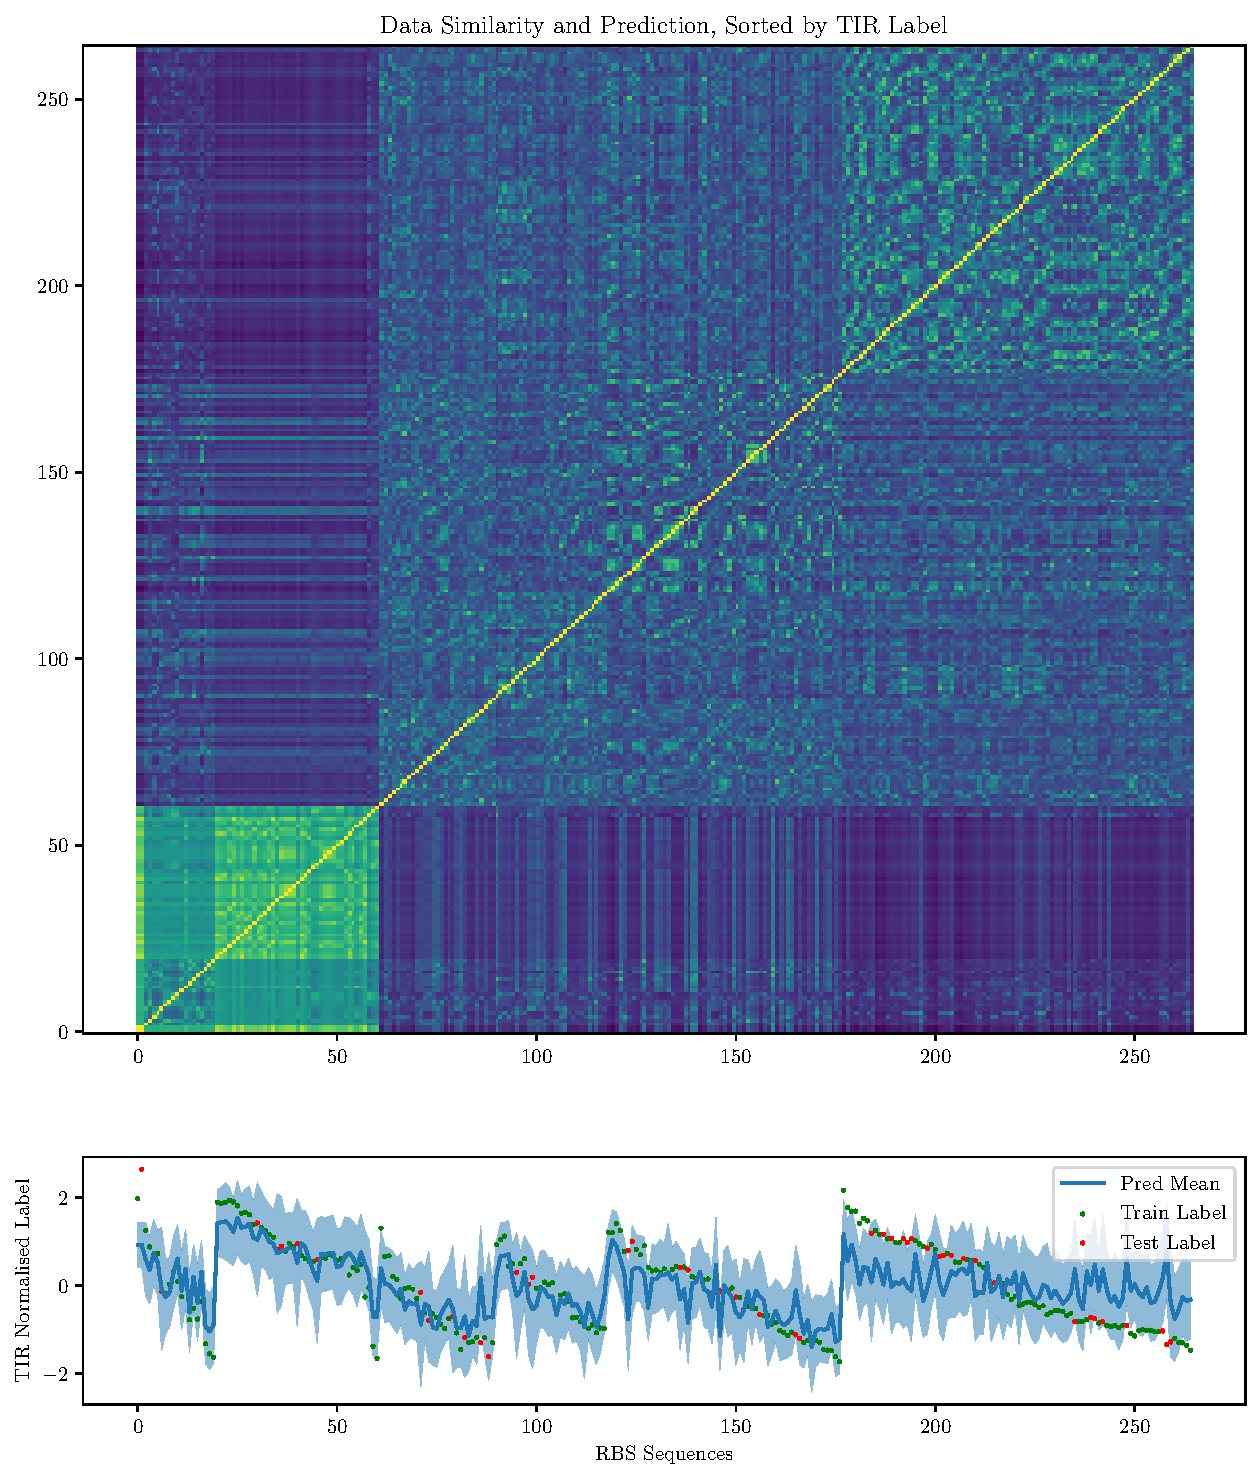
\includegraphics[scale = 0.3]{plots/Supplementary/Data_Similarity_and_Prediction_Sorted_by_TIR_Label.pdf}
    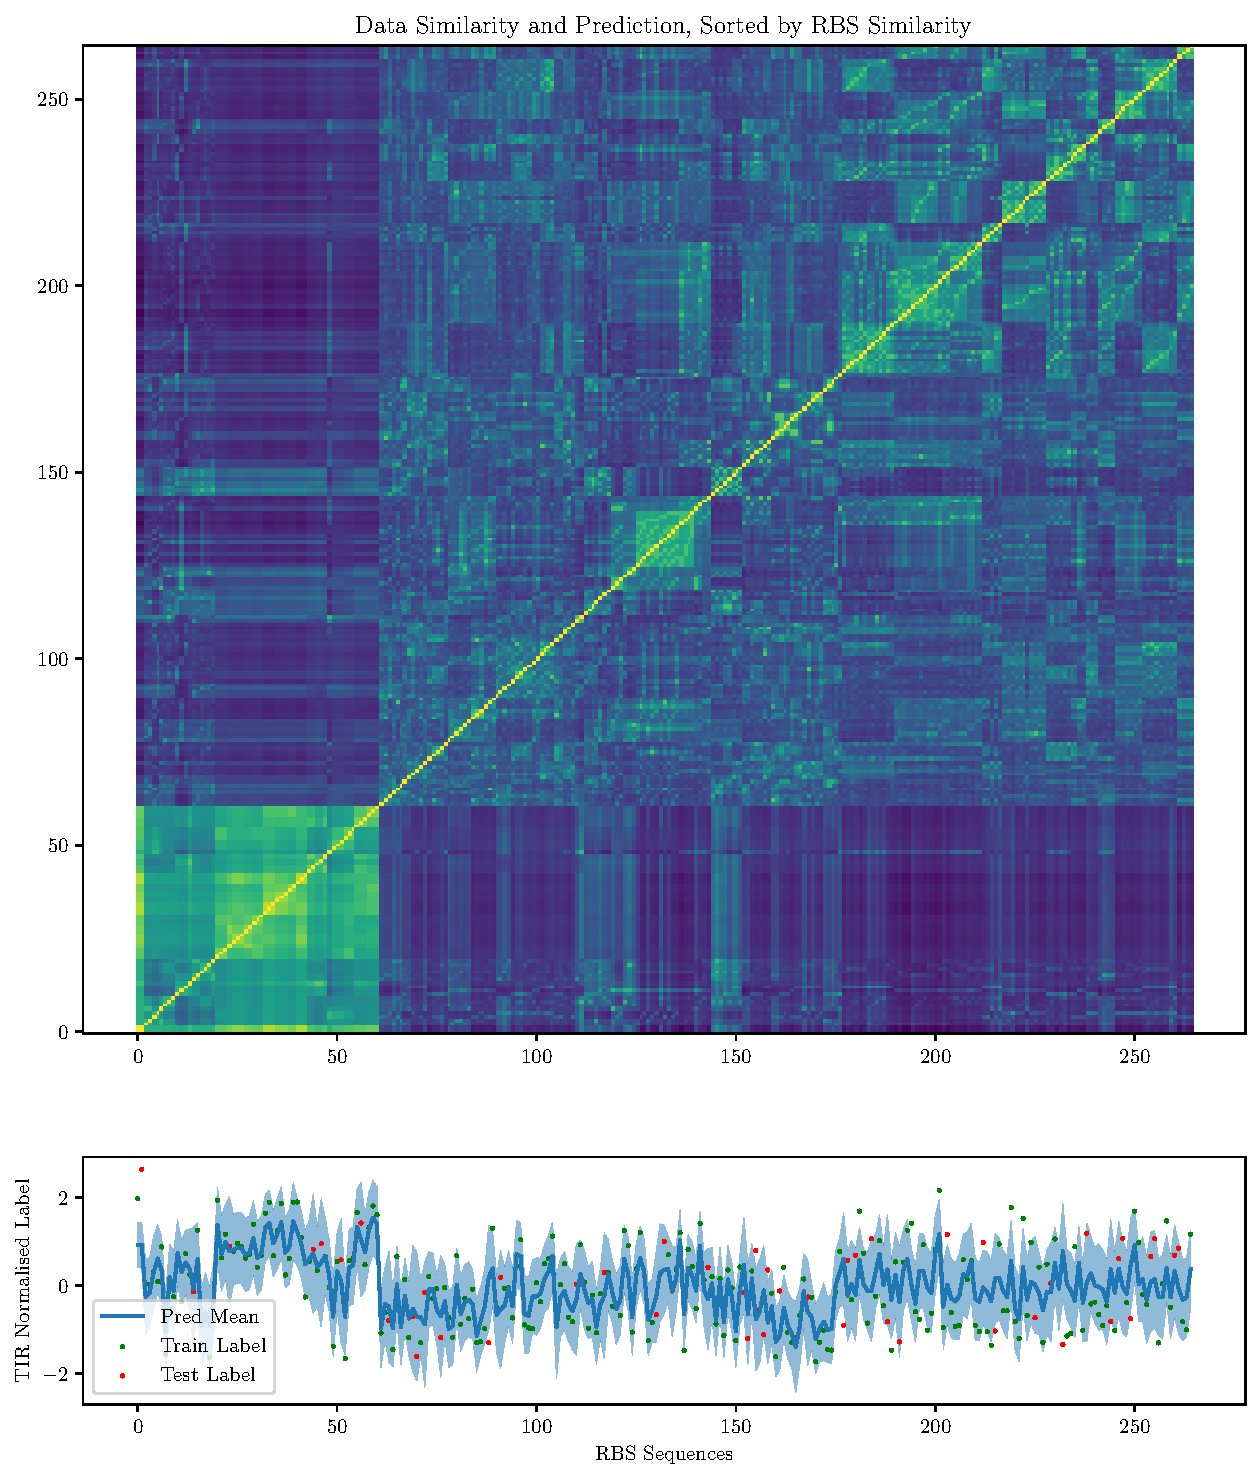
\includegraphics[scale = 0.3]{plots/Supplementary/Data_Similarity_and_Prediction_Sorted_by_RBS_Similarity.pdf}
    \caption{Kernel Heatmap and Predictions. Sequences are grouped as Consensus (1-2), BPS-C (3-20), BPS-NC (21-61), UNI (62-90), PPM (91-118), Bandit-0 (119-177), Bandit-1 (178-265). Inside of each group, sequences are clustered and sorted in terms of TIR labels (left) or RBS similarity (right). The first row shows the similarity measured by weighted degree kernel with shift, the second shows the predicted mean and uncertainty (1.95 standard deviation).}
    \label{fig:my_label}
\end{figure}

\begin{figure}
    \centering
    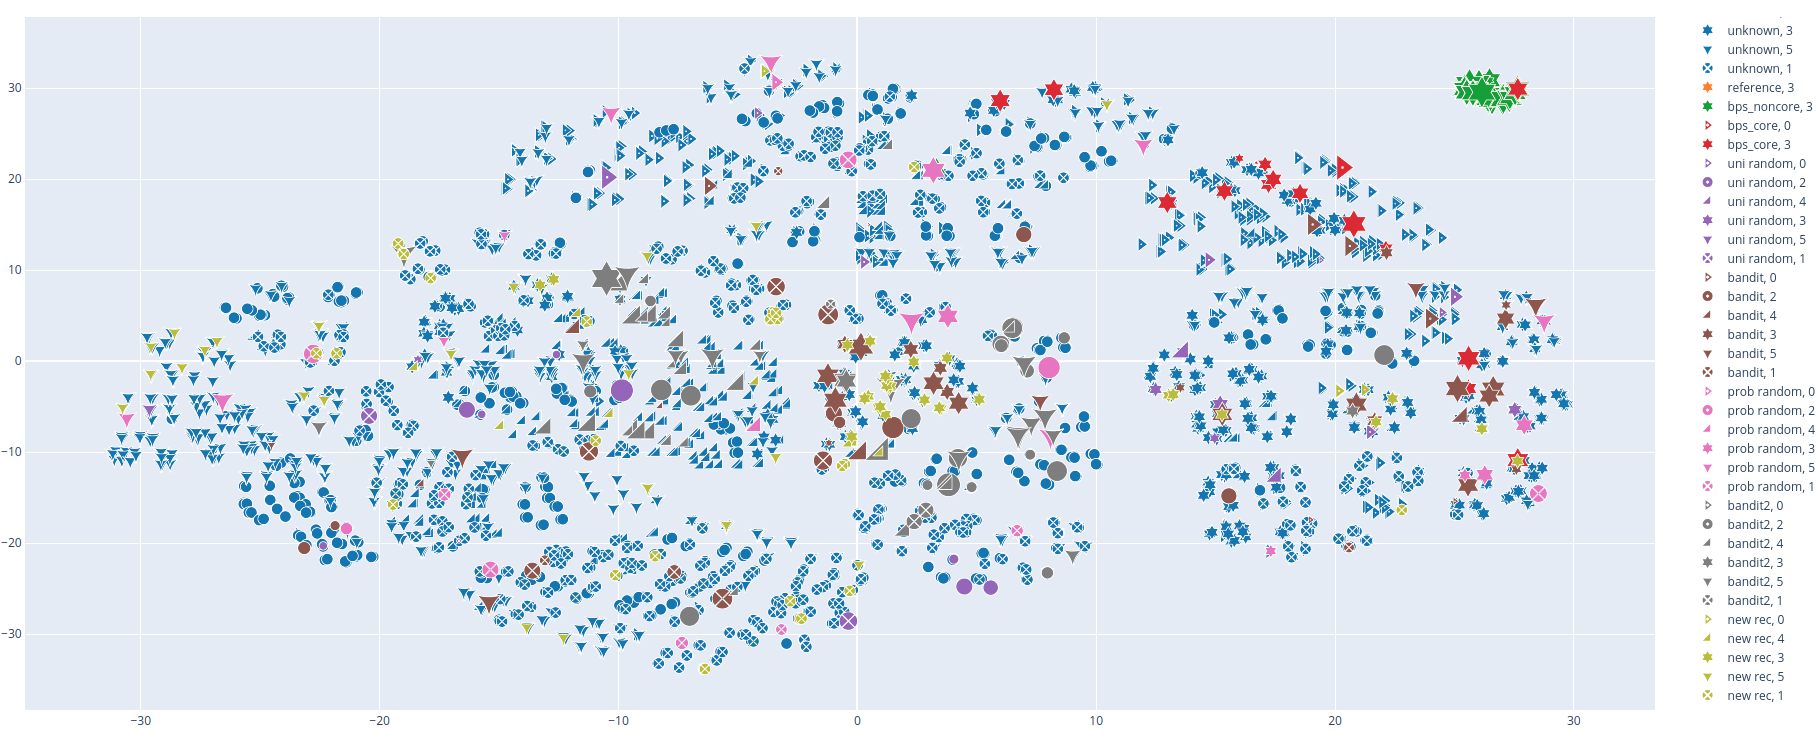
\includegraphics[scale = 0.25]{plots/Supplementary/clustering.png}
    \caption{TSNE of RBS sequences in design space with clustering. The distance is calculated based on the weighted degree kernel on RBS sequences. Colours indicate different groups, shapes indicate different clusters.}
    \label{fig:my_label}
\end{figure}

\subsection{Gaussian Process Regression}

A \textit{Gaussian process} is a collection of random variables, any finite number of which have a joint Gaussian distribution. 
We define mean function $\mu(\mathbf{x})$  and covariance function $k(\mathbf{x}, \mathbf{x}^\prime)$ of a real process $f(\mathbf{x})$ as
\begin{align}
    \mu(\mathbf{x}) &= \mathbb{E}[f(\mathbf{x})]\\
    k(\mathbf{x}, \mathbf{x}^\prime) &= \mathbb{E}[(f(\mathbf{x}) - \mu(\mathbf{x}))(f(\mathbf{x}^\prime) - \mu(\mathbf{x}^\prime))].
\end{align}

A Gaussian process is specified by its mean function and convariance function as $f(\mathbf{x}) \sim \mathcal{G} \mathcal{P}\left(\mu(\mathbf{x}), k\left(\mathbf{x}, \mathbf{x}^{\prime}\right)\right)$.
We consider the case where the observations are noisy, i.e. $\{(\mathbf{x}_i, y_i)| i = 1, \dots, n\}$, where $y_i = f(\mathbf{x}_i) + \epsilon$ with $\epsilon \sim \mathcal{N}(0, \alpha^2)$. 
The Gaussian noise is independent identically distributed, and the prior on the noisy observations is then $\operatorname{cov}\left(y_{p}, y_{q}\right)=k\left(\mathbf{x}_{p}, \mathbf{x}_{q}\right)+\alpha^{2} \delta_{p q}$,
where $\delta_{pq}$ is a Kronecker delta which is one if $p = q$ and zero otherwise.
It is equivalent to a diagonal matrix $\alpha^2 I$ on the kernel matrix evaluated on the training points.

For $n_\ast$ test points $X_\ast$, we assume the prior over the functions values as a random Gaussian vector $\mathbf{f}_\ast \sim \mathcal{N}(\mathbf{0}, K(X_\ast, X_\ast))$.
Then the joint distribution of the observed target values and the function values at the test points under the prior as 
\begin{align}
    \left[\begin{array}{l}\mathbf{y} \\ \mathbf{f}_{*}\end{array}\right] \sim \mathcal{N}\left(\mathbf{0},\left[\begin{array}{cc}K(X, X)+\alpha^{2} I & K\left(X, X_{*}\right) \\ K\left(X_{*}, X\right) & K\left(X_{*}, X_{*}\right)\end{array}\right]\right)
\end{align}
where $K(X, X_\ast)$ denotes the $n \times n_\ast$ covariance/Kernel matrix evaluated at all pairs of training and testing points, similarly for other kernel matrices.
Then the posterior of the test points (i.e. predictive distributions) is given by the conditional distribution $\mathbf{f}_\ast | X, \mathbf{y}, X_\ast \sim \mathcal{N}(\bar{\mathbf{f}}_\ast, cov(\mathbf{f}_\ast))$, where
\begin{align}
   \overline{\mathbf{f}}_{*} & \triangleq \mathbb{E}\left[\mathbf{f}_{*} \mid X, \mathbf{y}, X_{*}\right]=K\left(X_{*}, X\right)\left[K(X, X)+\alpha^{2} I\right]^{-1} \mathbf{y} \\
   \label{Eq: predicted variance}
   \operatorname{cov}\left(\mathbf{f}_{*}\right) &=K\left(X_{*}, X_{*}\right)-K\left(X_{*}, X\right)\left[K(X, X)+\alpha^{2} I\right]^{-1} K\left(X, X_{*}\right) 
\end{align}
For noisy test targets $\mathbf{y}_\ast$, we can compute the predictive distribution by adding $\alpha^2 I$ to the variance term $cov(\mathbf{f}_\ast)$ in Eq. (\ref{Eq: predicted variance}).
% We now introduce the marginal likelihood (or evidence) $p(\mathbf{y}|X)$, is which the integral of the likelihood times the prior 
% \begin{align}
%     p(\mathbf{y} \mid X)=\int p(\mathbf{y} \mid \mathbf{f}, X) p(\mathbf{f} \mid X) d \mathbf{f}
% \end{align}



\subsection{Choices of Kernels}

The choice of covariance function is critical for the performance of Gaussian process regression, we show a number of different string kernels tested in this study below:

\begin{itemize}
    \item \textit{Spectrum Kernel.}
    \begin{align}
        k_\ell^{\text{Spec}}(X, X^\prime) =\left\langle\phi_{\ell}^{\mathrm{Spec}}(\mathbf{x}), \phi_{\ell}^{\mathrm{Spec}}\left(\mathbf{x}^{\prime}\right)\right\rangle = \phi_{\ell}^{\mathrm{Spec}}(\mathbf{x})^T \phi_{\ell}^{\mathrm{Spec}}\left(\mathbf{x}^{\prime}\right).
    \end{align}
     where $\mathbf{x}, \mathbf{x}^\prime$ are two RBS sequences in $\mathcal{D}$ over an alphabet $\Sigma$. We denote the number of letters in the alphabet as $|\Sigma|$. 
    $\phi_{\ell}^{\mathrm{spec}}(\mathbf{x})$ maps the sequence $X$ into a $|\Sigma|^\ell$ dimensional feature space, where each dimension is the count of the number of one of the $|\Sigma|^\ell$ possible strings $s$ of length $\ell$. 
    Let $X, X^\prime$ be two metrics which include $n$ sequences, and $\Phi_d^{Spec}(X) \in \mathbb{R}^{n \times |\Sigma|^{\ell}}$, then the spectrum kernel over metrics is 
    \begin{align}
         K_\ell^{\text{Spec}}(X, X^\prime) = \Phi_{\ell}^{\mathrm{Spec}}(X) \Phi_{\ell}^{\mathrm{Spec}}\left(X^{\prime}\right)^T.
    \end{align}
    
    \item \textit{Sum of Spectrum Kernel,} considers weighted sum over different parts of the string. 
    
    \item \textit{Mixed Spectrum Kernel,} considers weighted sum over different substring length, with $\beta_d = \frac{2(\ell - d + 1)}{\ell(\ell+1)}$,
        \begin{align}
            k_\ell^{MixedSpec}(\mathbf{x}, \mathbf{x}^\prime) 
            = \sum_{d=1}^{\ell} \beta_d k_d^{Spec}(\mathbf{x}, \mathbf{x}^\prime)
        \end{align}
    \item \textit{Weighted Degree Kernel,} considers positional information. WD kernel counts the match of kmers at corresponding positions in two sequences.
    For sequences with fixed length $L$ and weighted degree kernel considers substrings starting at each position $l = 1, ..., L$, with $\beta_d = \frac{2(\ell - d + 1)}{\ell(\ell+1)}$, \\
    \begin{align}
        k_\ell^{WD}(\mathbf{x}, \mathbf{x}^\prime) 
        &= \sum_{d=1}^{\ell} \beta_d \sum_{l=1}^{L-d+1} \gamma_l k_d^{Spec}(\mathbf{x}_{[l:l+d]}, \mathbf{x}_{[l:l+d]}^\prime)\\
        &= \sum_{d=1}^{\ell} \beta_d \sum_{l=1}^{L-d+1} \gamma_l \phi_d^{Spec}(\mathbf{x}_{[l:l+d]})^T \phi_d^{Spec}(\mathbf{x}_{[l:l+d]}^\prime)\\
        &= \sum_{d=1}^{\ell} \beta_d \sum_{l=1}^{L-d+1} \gamma_l \mathbb{I}(\mathbf{x}_{[l:l+d]} = \mathbf{x}_{[l:l+d]}^\prime),
    \end{align}
    where $\mathbb{I}(\text{true}) = 1$ and 0 otherwise. 
    
    \item \textit{Weighted Degree Kernel With Shift.}
    \begin{align}
        k_\ell^{WDS}(\mathbf{x}, \mathbf{x}^\prime) 
        &= \sum_{d=1}^{\ell} \beta_d \sum_{l=1}^{L-d+1} \gamma_l \sum_{s = 0, s + l \leq L}^{S(l)} \delta_s
        \left(k_d^{Spec}(\mathbf{x}_{[l+s:l+s+d]}, \mathbf{x}_{[l:l+d]}^\prime) + (k_d^{Spec}(\mathbf{x}_{[l:l+d]}, \mathbf{x}_{[l+s:l+s+d]}^\prime)\right)\\
        &= \sum_{d=1}^{\ell} \beta_d \sum_{l=1}^{L-d+1} \gamma_l \sum_{s = 0, s + l \leq L}^{S(l)} \delta_s
        \left(\mathbb{I}(\mathbf{x}_{[l+s:l+s+d]} = \mathbf{x}_{[l:l+d]}^\prime) + (\mathbb{I}(\mathbf{x}_{[l:l+d]}= \mathbf{x}_{[l+s:l+s+d]}^\prime)\right),
    \end{align}
    where $\beta_d = \frac{2(\ell - d + 1)}{\ell(\ell+1)}, \delta_s = \frac{1}{2(s+1)}$, $\gamma_l$ is a weighting over the position in the
    sequence, where we choose to use a uniform weighting over the sequences, i.e. $\gamma_l = 1/L$. $S(l)$ determines the shift
    range at position $l$.
\end{itemize}

\textbf{From kernel to distance}:
$$d(\mathbf{x}, \mathbf{x}^\prime) = \sqrt{k(\mathbf{x}, \mathbf{x}) + k(\mathbf{x}^\prime, \mathbf{x}^\prime) - 2 k(\mathbf{x}, \mathbf{x}^\prime)} $$

\subsubsection{Normalisation of Kernel}

As part of data pre-processing,
the range of all features should be normalised so that each feature contributes approximately proportionately to the predictive model. 
The kernel matrix is represented by the inner product of the underlying feature vectors, it needs to be normalised before being used in the downstream regression models. 
Up-scaling (down-scaling) features can be understood as down-scaling (up-scaling) regularizers such that they penalise the features less (more). 

Here we consider two approaches for kernel normalisation: centering and unit norm. 
We will show how to convert the normalisation in terms of feature vectors to normalisation in terms of kernel matrices. 
As defined before, consider $\mathbf{x}, \mathbf{x}^\prime$ are two RBS sequences in $\mathcal{D}$ over an alphabet $\Sigma$.
We denote $\phi(\mathbf{x}_i)$ as a column feature vector of sequence $\mathbf{x}_i$, 
where a feature function $\phi: \mathbf{x} \rightarrow \mathbb{R}^d$. Assume there is total of $n$ sequences in the data $X$ ($n'$ sequences in the data $X'$). 
We illustrate centering and unit norm normalisation below. 

\begin{itemize}
    \item Centering. 
    Defining the mean vector as $\bar{\Phi}(X) = \frac{1}{n} \sum_{s = 1}^n \phi(\mathbf{x}_s) \in \mathbb{R}^d$, the centered feature vector $\phi^C(\mathbf{x}_i) \in \mathbb{R}^d$ of $\mathbf{x}_i$ is
    \begin{align}
        \phi^{C}(\mathbf{x}_i) = \phi(\mathbf{x}_i) - \bar{\Phi}(X) = \phi(\mathbf{x}_i) - \frac{1}{n'} \sum_{s = 1}^{n'} \phi(\mathbf{x}_s).
    \end{align}
    The corresponding centering kernel value between $\mathbf{x}_i$ and $\mathbf{x}_j$ is then 
    \begin{align}
        k^C(\mathbf{x}_i, \mathbf{x}_j) &= <\phi^C(\mathbf{x}_i), \phi^C(\mathbf{x}_j)>\\
        &= \left( \phi(\mathbf{x}_i) - \frac{1}{n} \sum_{s = 1}^n \phi(\mathbf{x}_s)\right)^T \left( \phi(\mathbf{x}_j) - \frac{1}{n'} \sum_{s' = 1}^{n'} \phi(\mathbf{x}_{s'})\right)\\
        &= \phi(\mathbf{x}_i)^T \phi(\mathbf{x}_j) - \left( \frac{1}{n} \sum_{s = 1}^n \phi(\mathbf{x}_s)\right)^T \phi(\mathbf{x}_j) - \phi(\mathbf{x}_i)^T \left(\frac{1}{n} \sum_{s' = 1}^{n'} \phi(\mathbf{x}_{s'})\right) + \left( \frac{1}{n} \sum_{s = 1}^n \phi(\mathbf{x}_s)\right)^T \left(\frac{1}{n'} \sum_{s' = 1}^{n'} \phi(\mathbf{x}_{s'})\right)\\
        &= k(\mathbf{x}_i, \mathbf{x}_j) - \frac{1}{n} \sum_{s=1}^n k(\mathbf{x}_s, \mathbf{x}_j) - \frac{1}{n'} \sum_{s'=1}^{n'} k(\mathbf{x}_i, \mathbf{x}_{s'}) + \frac{1}{n^2} \sum_{s = 1}^n \sum_{s'=1}^{n'} k(\mathbf{x}_s, \mathbf{x}_{s'})
    \end{align}
    
    \item Unit Norm. Define the ($l_2$) norm of a feature vector as $||\phi(\mathbf{x})|| = \sqrt{\sum_{m = 1}^d \phi_d(\mathbf{x})^2} = \sqrt{k(\mathbf{x}, \mathbf{x})} \in \mathbb{R}^+$, then the unit norm feature vector $\phi^{UN}(\mathbf{x}_i) \in \mathbb{R}^d$ of $\mathbf{x}_i$ is 
    \begin{align}
        \phi^{UN}(\mathbf{x}_i) = \frac{\phi(\mathbf{x}_i)}{||\phi(\mathbf{x}_i)||}.
    \end{align}
    The corresponding unit norm kernel value between $\mathbf{x}_i$ and $\mathbf{x}_j$ is then 
    \begin{align}
        k^{UN}(\mathbf{x}_i, \mathbf{x}_j) &= <\frac{\phi(\mathbf{x}_i)}{||\phi(\mathbf{x}_i)||}, \frac{\phi(\mathbf{x}_j)}{||\phi(\mathbf{x}_j)||}>\\
        &= \frac{\phi(\mathbf{x}_i)^T \phi(\mathbf{x}_j)}{||\phi(\mathbf{x}_i)|| \times ||\phi(\mathbf{x}_j)||}\\
        &= \frac{k(\mathbf{x}_i, \mathbf{x}_j)}{\sqrt{k(\mathbf{x}_i, \mathbf{x}_i)  k(\mathbf{x}_j, \mathbf{x}_j)}}
    \end{align}
    
     \item Unit Variance. 
    After the centering and unit norm normalisation, the kernel matrix is unit variance as well. 
    In the following, we show transformations of the unit variance (with centering) normalisation.
    Define the variance vector ${Var}(\Phi(X)) = \frac{1}{n} \sum_{s=1}^n ||\phi(\mathbf{x}_s) - \bar{\Phi}(X)||^2 = \frac{1}{n} \sum_{s=1}^n ||\phi(\mathbf{x}_s) - \sum_{s'=1}^n \left(\phi(\mathbf{x}_s')\right)||^2 = \frac{1}{n} \sum_{s=1}^n  k^C(\mathbf{x}_s, \mathbf{x}_s)  \in \mathbb{R}$, the unit variance feature vector $\phi^{UV}(\mathbf{x}_i) \in \mathbb{R}^d$ of $\mathbf{x}_i$ is
    \begin{align}
        \phi^{UV}(\mathbf{x}_i) = \frac{\phi(\mathbf{x}_i)}{\sqrt{Var(\Phi(X))}}.
    \end{align}
    The corresponding kernel representation is 
    \begin{align}
        k^{UV}(\mathbf{x}_i, \mathbf{x}_j) &= <\frac{\phi(\mathbf{x}_i)}{\sqrt{Var(\Phi(X))}}, \frac{\phi(\mathbf{x}_j)}{\sqrt{Var(\Phi(X'))}}>\\
        &= \frac{\phi(\mathbf{x}_i)^T \mathbf{x}_j}{\sqrt{Var(\Phi(X)) Var(\Phi(\mathbf{X'}))}}\\
        &= \frac{k(\mathbf{x}_i, \mathbf{x}_j)}{\sqrt{ \frac{1}{n} \sum_{s=1}^n  k^C(\mathbf{x}_s, \mathbf{x}_s)  \frac{1}{n} \sum_{s'=1}^{n'}  k^C(\mathbf{x}_{s'}, \mathbf{x}_{s'})}}
    \end{align}
    After centering and unit norm, $ \frac{1}{n} \sum_{s=1}^n  k^C(\mathbf{x}_s, \mathbf{x}_s) = k(\mathbf{x}_i, \mathbf{x}_i)$, which implies that after centering and unit norm, the kernel matrix is already unit variance normalised. 
\end{itemize}
For the Gaussian Process regression, we make of use of two kernel matrices: the kernel function between the training data itself, i.e. $K(X_{train}, X_{train})$; and
the kernel function taking the training data and testing data as inputs, i.e. $K(X_{test}, X_{train})$. 
%It is straightforward to normalise a square kernel which same input, i.e. $n = n'$ and $k(\mathbf{x}_i, \mathbf{x}_i),  k(\mathbf{x}_j, \mathbf{x}_j)$ taken from the diagonal of the matrix. 
%The second one (between train and test) is a little bit tricky. The different is not only that $n \neq n'$. 
We will state two ways of normalisation those two kind of matrices:
\begin{itemize}
    \item Normalise training and testing data separately.
    This approach is preferred for most of the machine learning algorithms since it follows the rule that we have no information about testing data while training.
    Then for centering, one should subtract the mean vector over the training data for both kinds of matrices.
    For unit norm normalisation, when one calculates $K^{UN}(X_{test}, X_{train})$, the two terms inside of square root: $k(\mathbf{x}_i, \mathbf{x}_i)$ is taken from $K(X_{test}, X_{test})[i,i]$, and $k(\mathbf{x}_j, \mathbf{x}_j)$ is taken from $K(X_{train}, X_{train})[j,j]$.
    
    \item Normalise training and testing data together, i.e. normalise $K(X_{train+test}, X_{train+test})$, then extra the parts we need from the normalised matrix. 
    This approach is suitable in a case where one already knows the whole of testing features. 
    For centering, one should subtract the mean vector over the whole matrix $\Phi(X_{train+test})$. 
    The unit norm normalisation is the same as in the previous case. 
\end{itemize}

For our experiment, we fix the design space before training, i.e. the testing features are already known before testing. 
So we choose to normalise the kernel matrix over the training and testing data together,
by first applying centering and then unit norm normalisation. 

\subsection{Batch Recommendation}

For recommending RBS sequences to label, we consider the Upper Confidence Bound (UCB) algorithm, 
%which is based on the \textit{optimism in the face of uncertainty}, 
selecting RBS sequences with the maximum upper confidence bound at round $t$, i.e.
\begin{align}
\label{Eq: GPUCB}
    \operatorname{argmax}_{\mathbf{x}_i \in \mathcal{D}} \left( \mu_{t-1}(\mathbf{x}_i) + \beta_t \sigma_{t-1}(\mathbf{x}_i)\right),
\end{align}
where $\beta_t$ is a hyperparmeter balancing the exploitation and exploration, 
$\mu_t(\mathbf{x}_i), \sigma_t(\mathbf{x}_i)$ are the predicted mean and standard deviation at round $t$ for the sequence $\mathbf{x}_i$.

Since labelling sequences is time-consuming, it is unrealistic to recommend sequence sequentially (i.e. one-by-one) and waiting for the label after each prediction.
Therefore we consider recommending sequences in batch and using Gaussian Process Batch Upper Confidence Bound (GP-BUCB) algorithm  \cite{desautels2012parallelizing}.
With batches of size $B$, the feedback mapping $fb[t] = \lfloor(t-1) / B\rfloor B$, i.e. 
\begin{align}
    \mathrm{fb}[t]=\left\{\begin{array}{cl}
    0 & : t \in\{1, \ldots, B\} \\
    B & : t \in\{B+1, \ldots, 2 B\} \\
    2 B & : t \in\{2 B+1, \ldots, 3 B\} \\
    & \vdots
    \end{array}\right.
\end{align}


A key property of Gaussian Process regression is that the predictive variance in Eq. (\ref{Eq: predicted variance}) only depends on observed points (i.e. features), but not on the labels of these observed points. 
So one can compute the posterior variance without actually observing the labels. 
The GP-BUCB policy is to select sequences that
\begin{align}
    \operatorname{argmax}_{\mathbf{x}_i \in \mathcal{D}} \left( \mu_{fb[t]}(\mathbf{x}_i) + \beta_t \sigma_{t-1}(\mathbf{x}_i)\right).
\end{align}
And only update $y_{t^{\prime}}=f\left(\boldsymbol{x}_{t^{\prime}}\right)+\varepsilon_{t^{\prime}} \text { for } t^{\prime} \in\{\mathrm{fb}[t]+1, \ldots, \mathrm{fb}[t+1]\}$ at the end of each batch ($\mathrm{fb}[t]<\mathrm{fb}[t+1]$). 
This is equivalent to sequential GP-UCB with \textit{hallucinated observations} $\boldsymbol{y}_{\mathrm{fb}[t]+1: t-1}=\left[\mu_{\mathrm{fb}[t]}\left(\boldsymbol{x}_{\mathrm{fb}[t]+1}\right), \ldots, \mu_{\mathrm{fb}[t]}\left(\boldsymbol{x}_{t-1}\right)\right]$, while the posterior variance decreases. 


\subsection{Design Pipeline}

The n + 1 round design is based on the nth round result, where each sequence has 6 replicates with TIR labels.
We pre-processed the data by taking a logarithm transformation and standardisation of the raw TIR label for each replicates respectively, where TIR is calculated as a derivative of GFP fluoresence divided by OD600 of culture over 4h counting from the start of log phase of growth. 
After normalisation, each replicate has zero mean and unit variance. 

For prediction, we use Gaussian process regression, with training on all normalised replicates and predicting on the design space (6-base core part design) except known sequences. 
We assume the observation are noisy, where the noise is under centered normal distribution with standard deviation $\alpha$.  
We model the covariance matrix using the weighted degree kernel with shift. 
We normalise the kernel with centering and unit norm in terms of the whole kernel constructed by both first round result and design space. 
The hyperparameter for kernel, including maximum substring length  $l$, maximum shift length $s$, and the noise standard deviation $\alpha$ of Gaussian process model are choose based on 10-repeat 5-fold cross validation. 
We choose $l=6, s= 1, \alpha = 2$ for the second round design. 

For recommendation, we use batch upper confidence bound introduced by GP-BUCB algorithm \cite{desautels2012parallelizing}. 
The upper confidence bound is constructed by predicted mean plus 2 predicted standard deviation.   
We recommend 90 sequences from the design space. 



\subsection{Intuition behind UCB and visualisation}

\begin{itemize}
    \item Exploitation and exploration explanation.
    \item Visualise coverage by clustering plot.
    \item Table for in-clustering mean and variance.
\end{itemize}

\subsection{Result analysis}

\begin{itemize}
    \item violinplot.
    \item regression performance plot, table.
    \item kernel matrix plot.
\end{itemize}

\subsection{Statistics of the core vs non-core regions of the RBS}

In our study, we have tested a set of sequnces designed to confirm the notion that changing bases within the RBS core (6 bases) is statistically more influencing the TIR than the changes made outside the core.
This hypothesis has been build based on reported biases towards certain bases present in the core of the RBS but absent outside of it.
For example, according to \cite{SHULTZABERGER2001} there is a strong bias towards A and G bases in the core region of the RBS.
Similarly outside of the 6 bases of the core in the wider 20 bp context of the RBS there is no significant bias towards any particular base which suggest that these bases do not contribute to the overal TIR of a given RBS. 
This effect is shown in (Figure \ref{fig:core_vs_noncore}), which shows results for our set X of sequences.
The value of Welch's t-test between the mean TIR in core and non-core groups is -4.8780 with p-value < 0.0001 and 34 degrees of Freedom.

\begin{figure}[h]
    \centering
    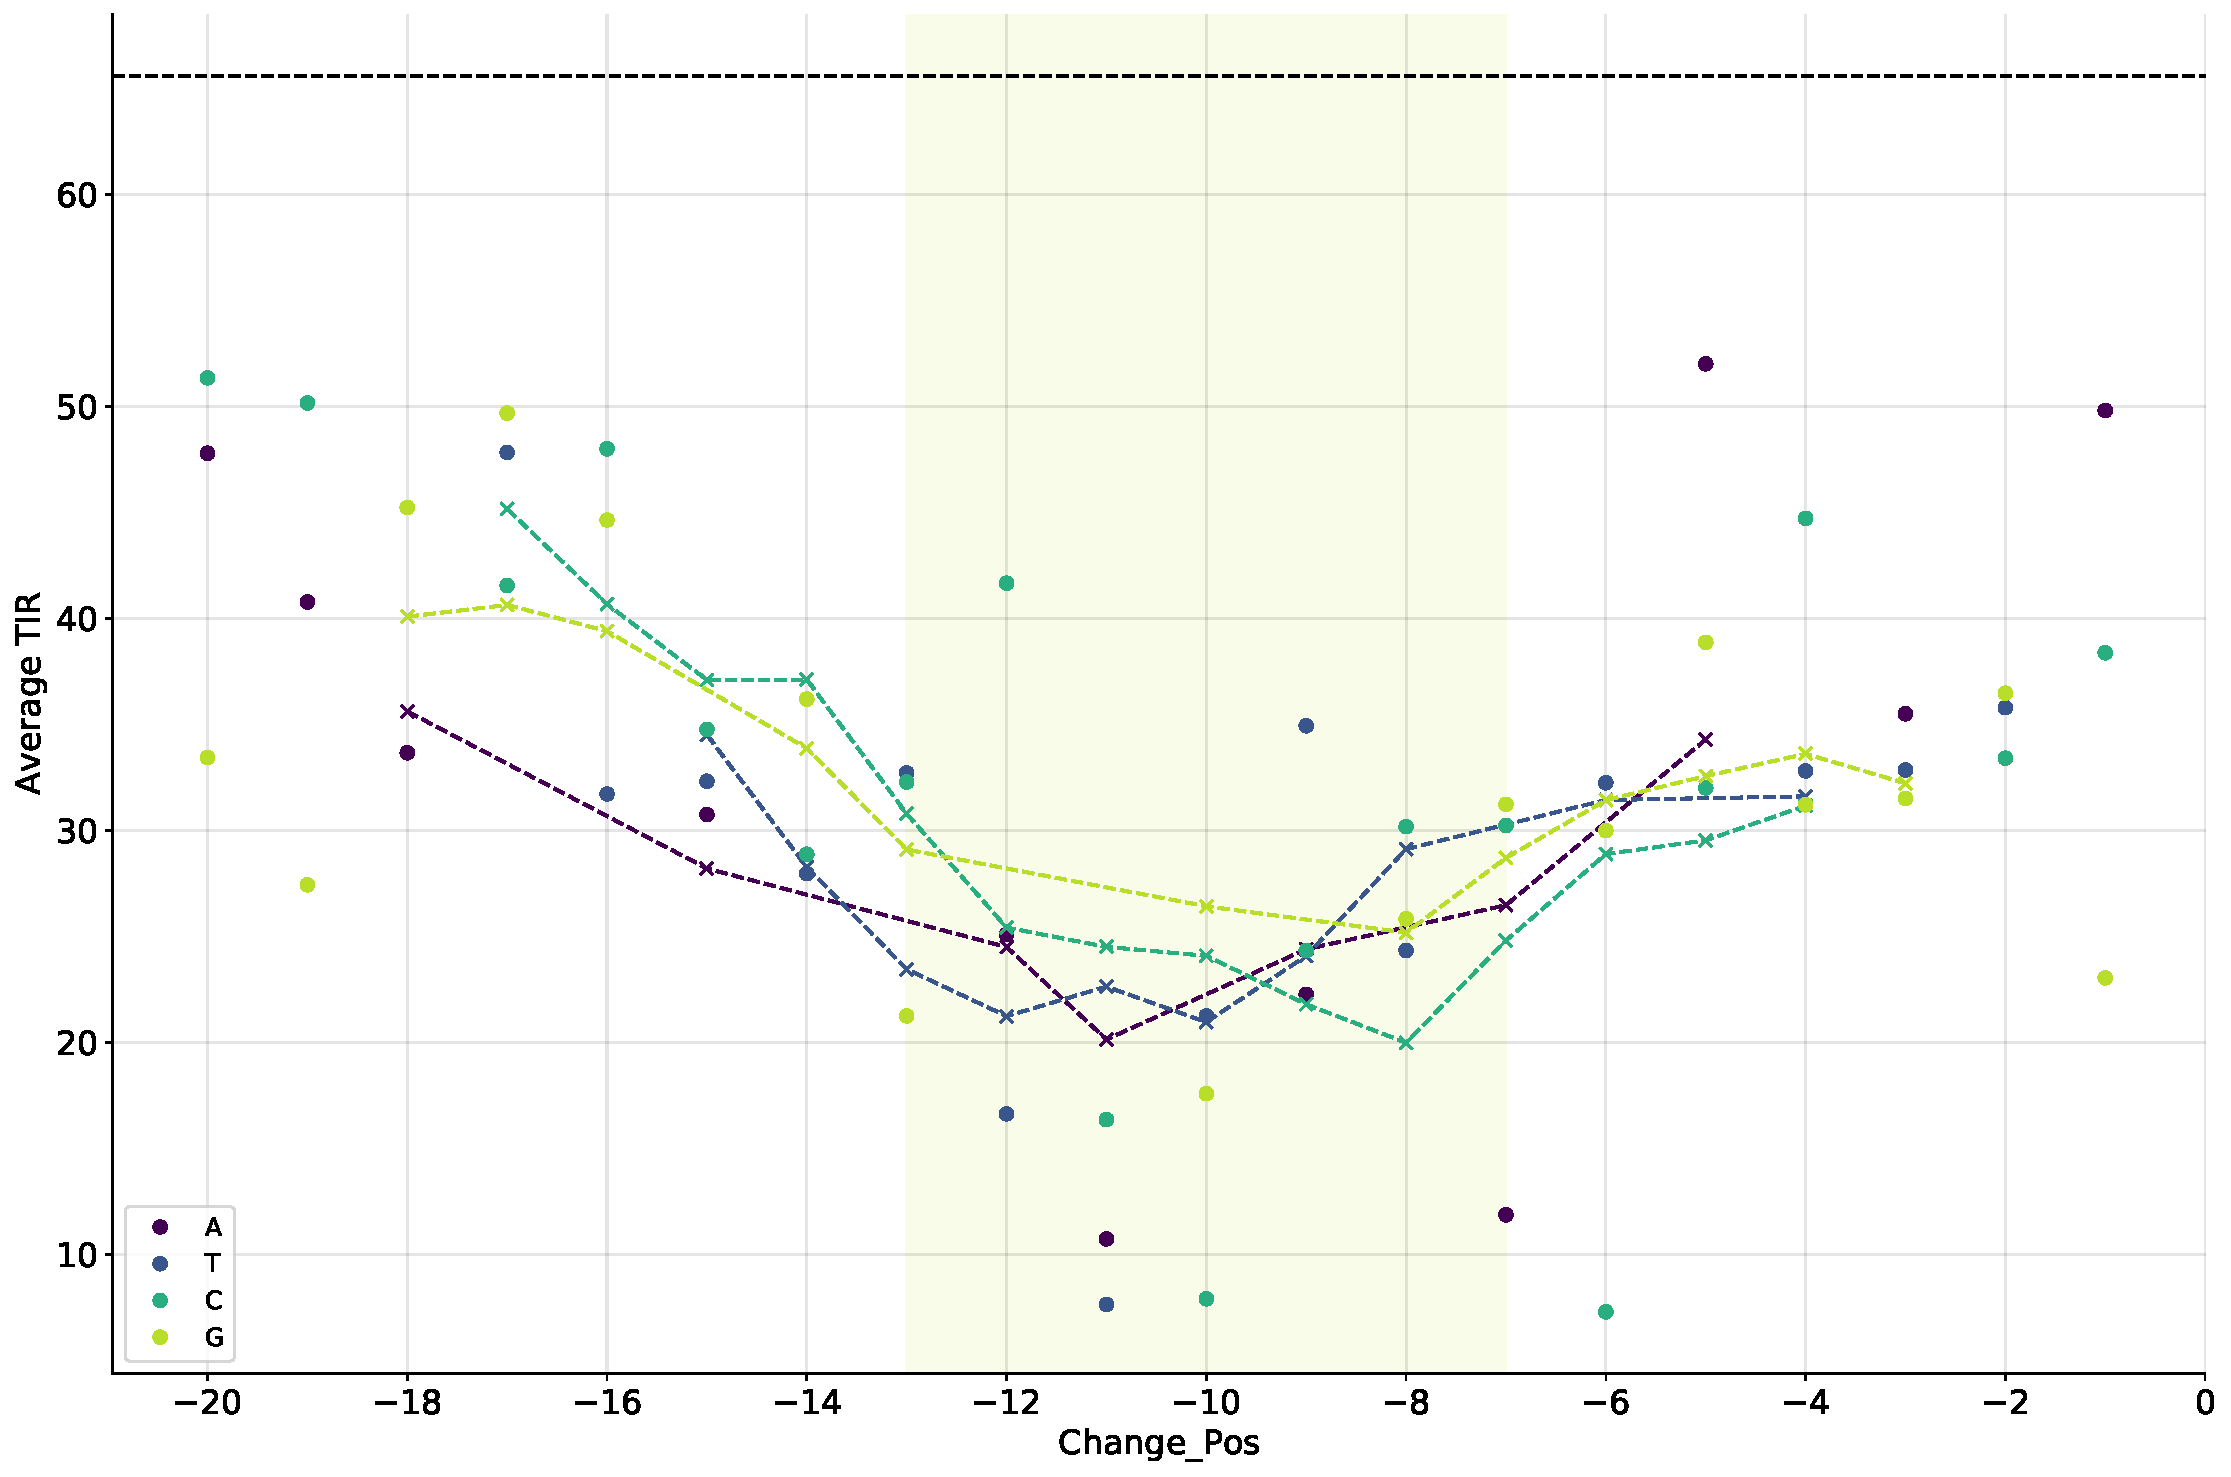
\includegraphics[scale=0.4]{plots/Supplementary/core_vs_noncore.pdf}
    \caption{\textbf{Comparison of base change impact on TIR in core versus non-core region.} The core region is highligthed in light green and the lines are rolling averages for each base. The top dotted line shows the TIR for the benchmark sequence, where dots represent a change at a given position to a given base, which is colour coded.}
    \label{fig:core_vs_noncore}
\end{figure}

\section{Supplementary Figures}

\begin{figure}
     \centering
     \begin{subfigure}[b]{0.49\textwidth}
         \centering
         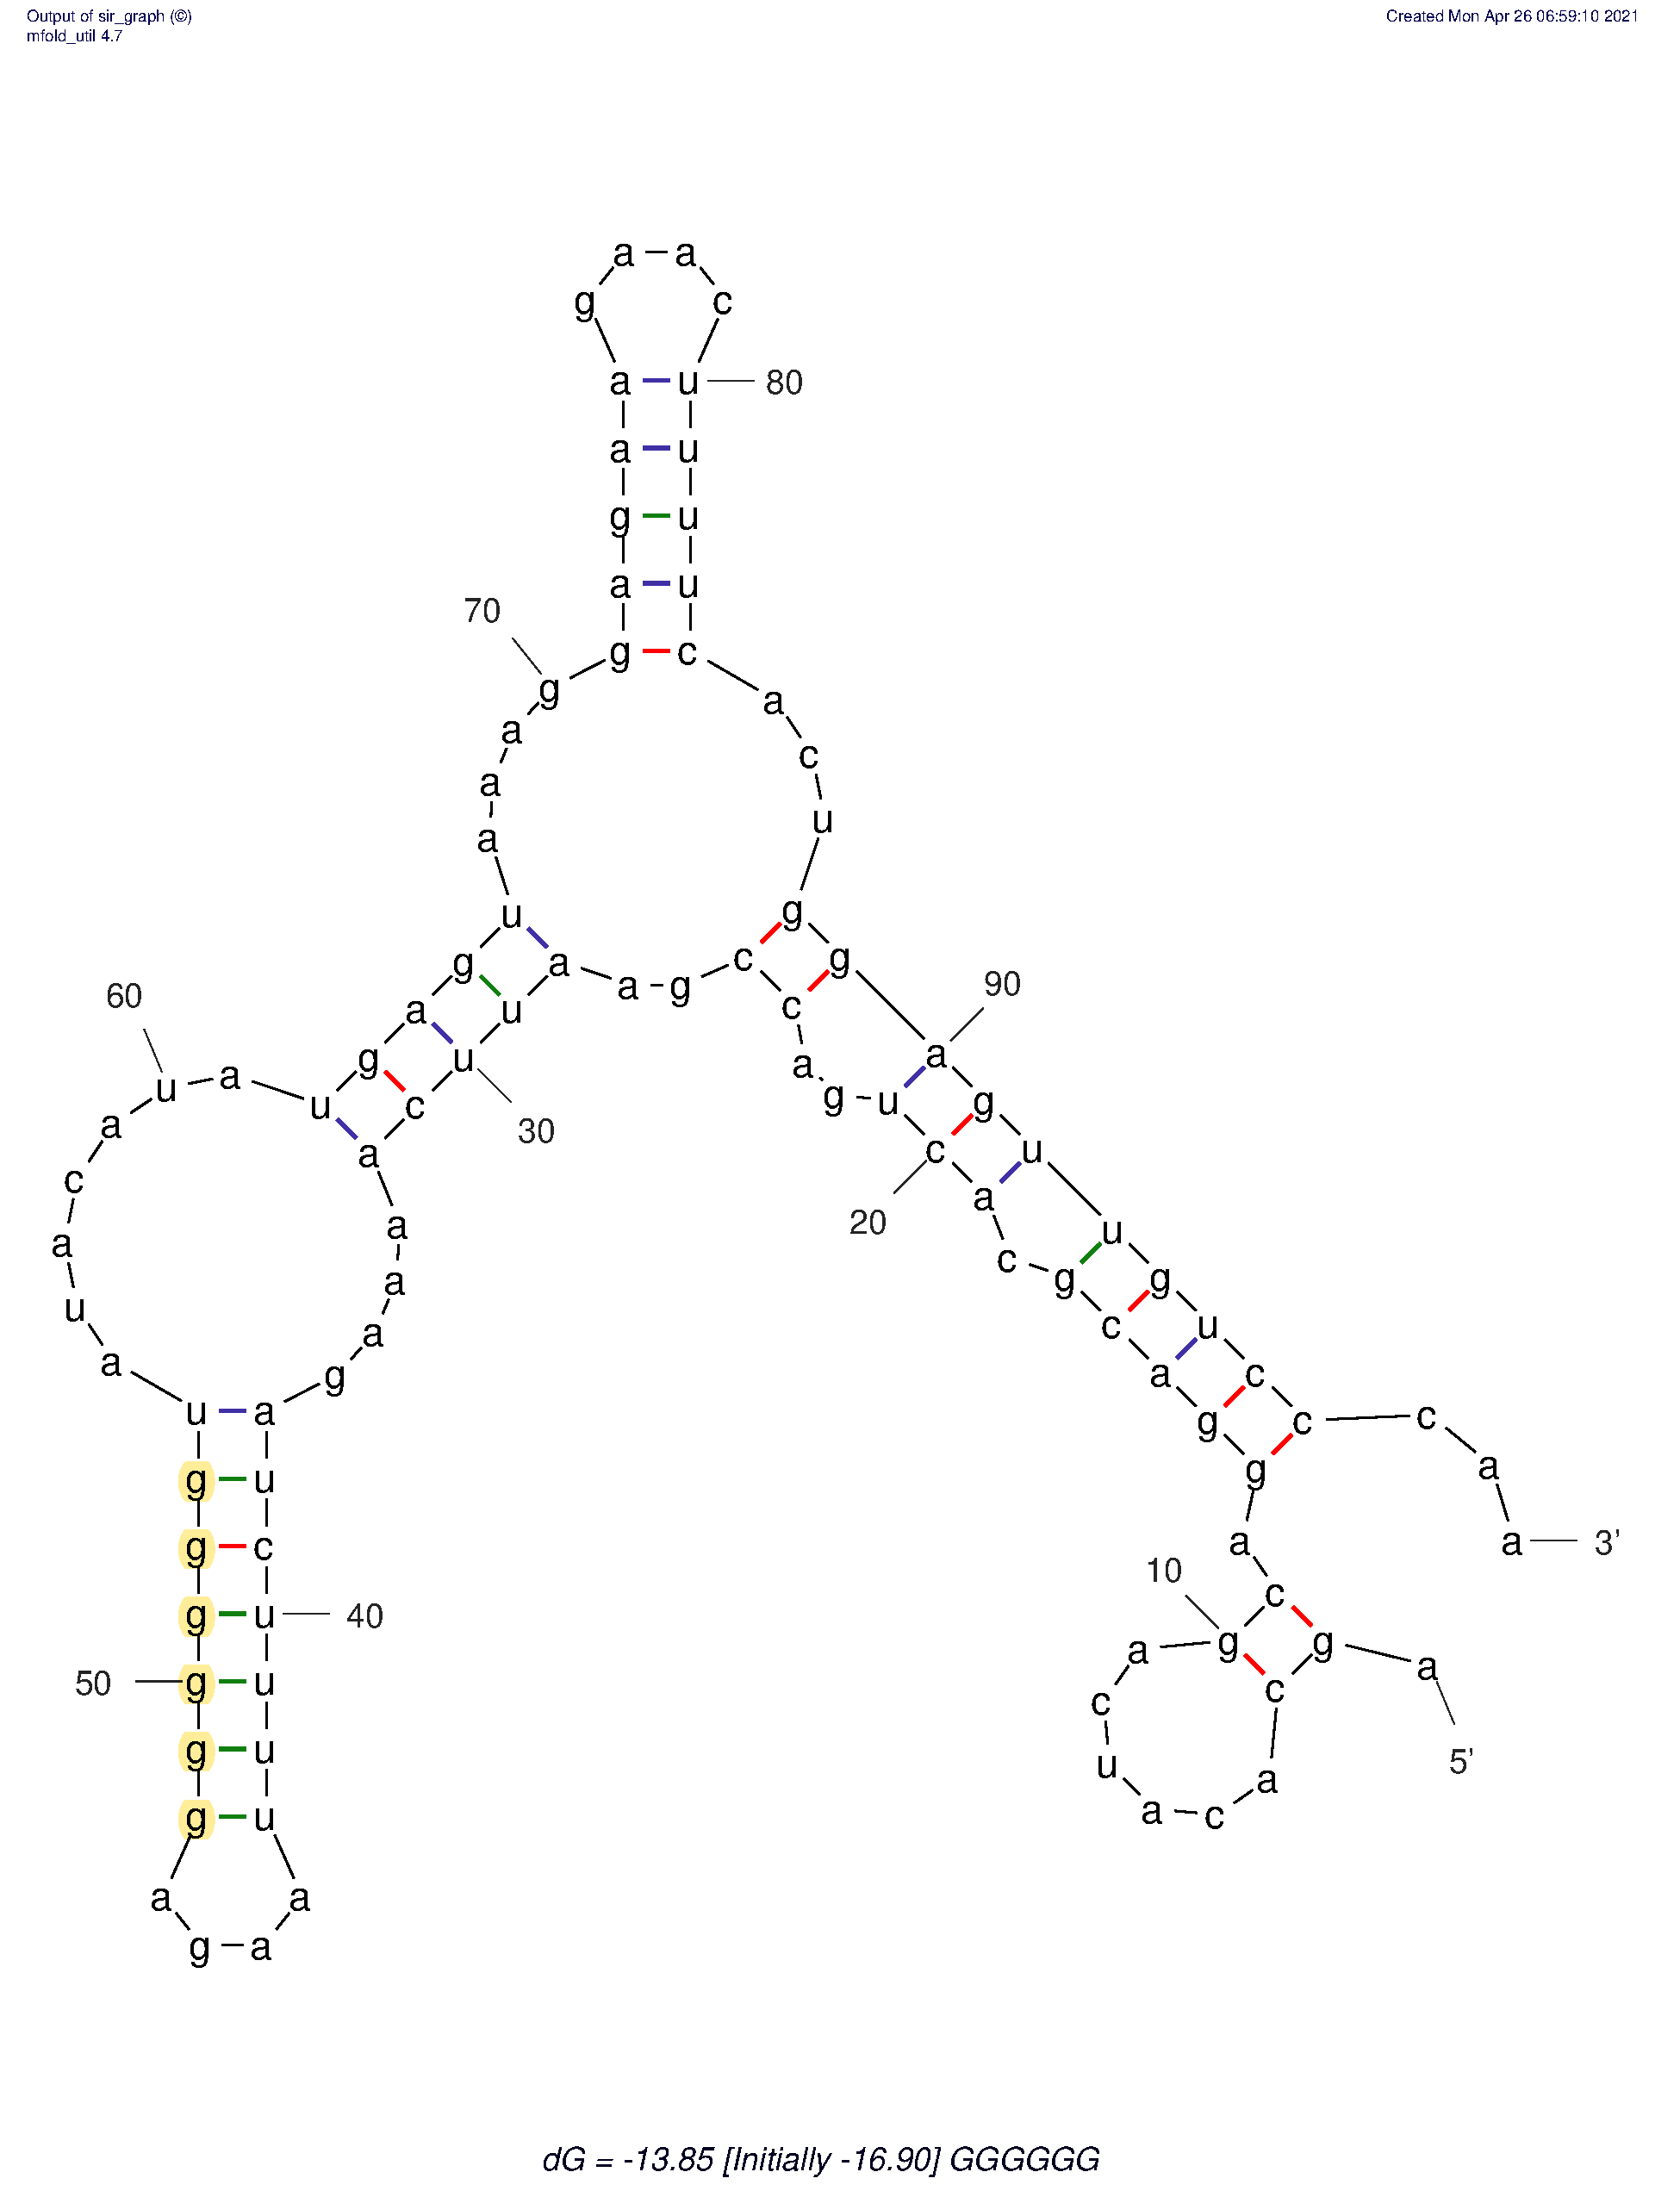
\includegraphics[scale=0.25]{plots/Supplementary/Structure GGGGGG.pdf}
         \caption{$y=x$}
         \label{fig:GGGGGG}
     \end{subfigure}
     \hfill
     \begin{subfigure}[b]{0.49\textwidth}
         \centering
         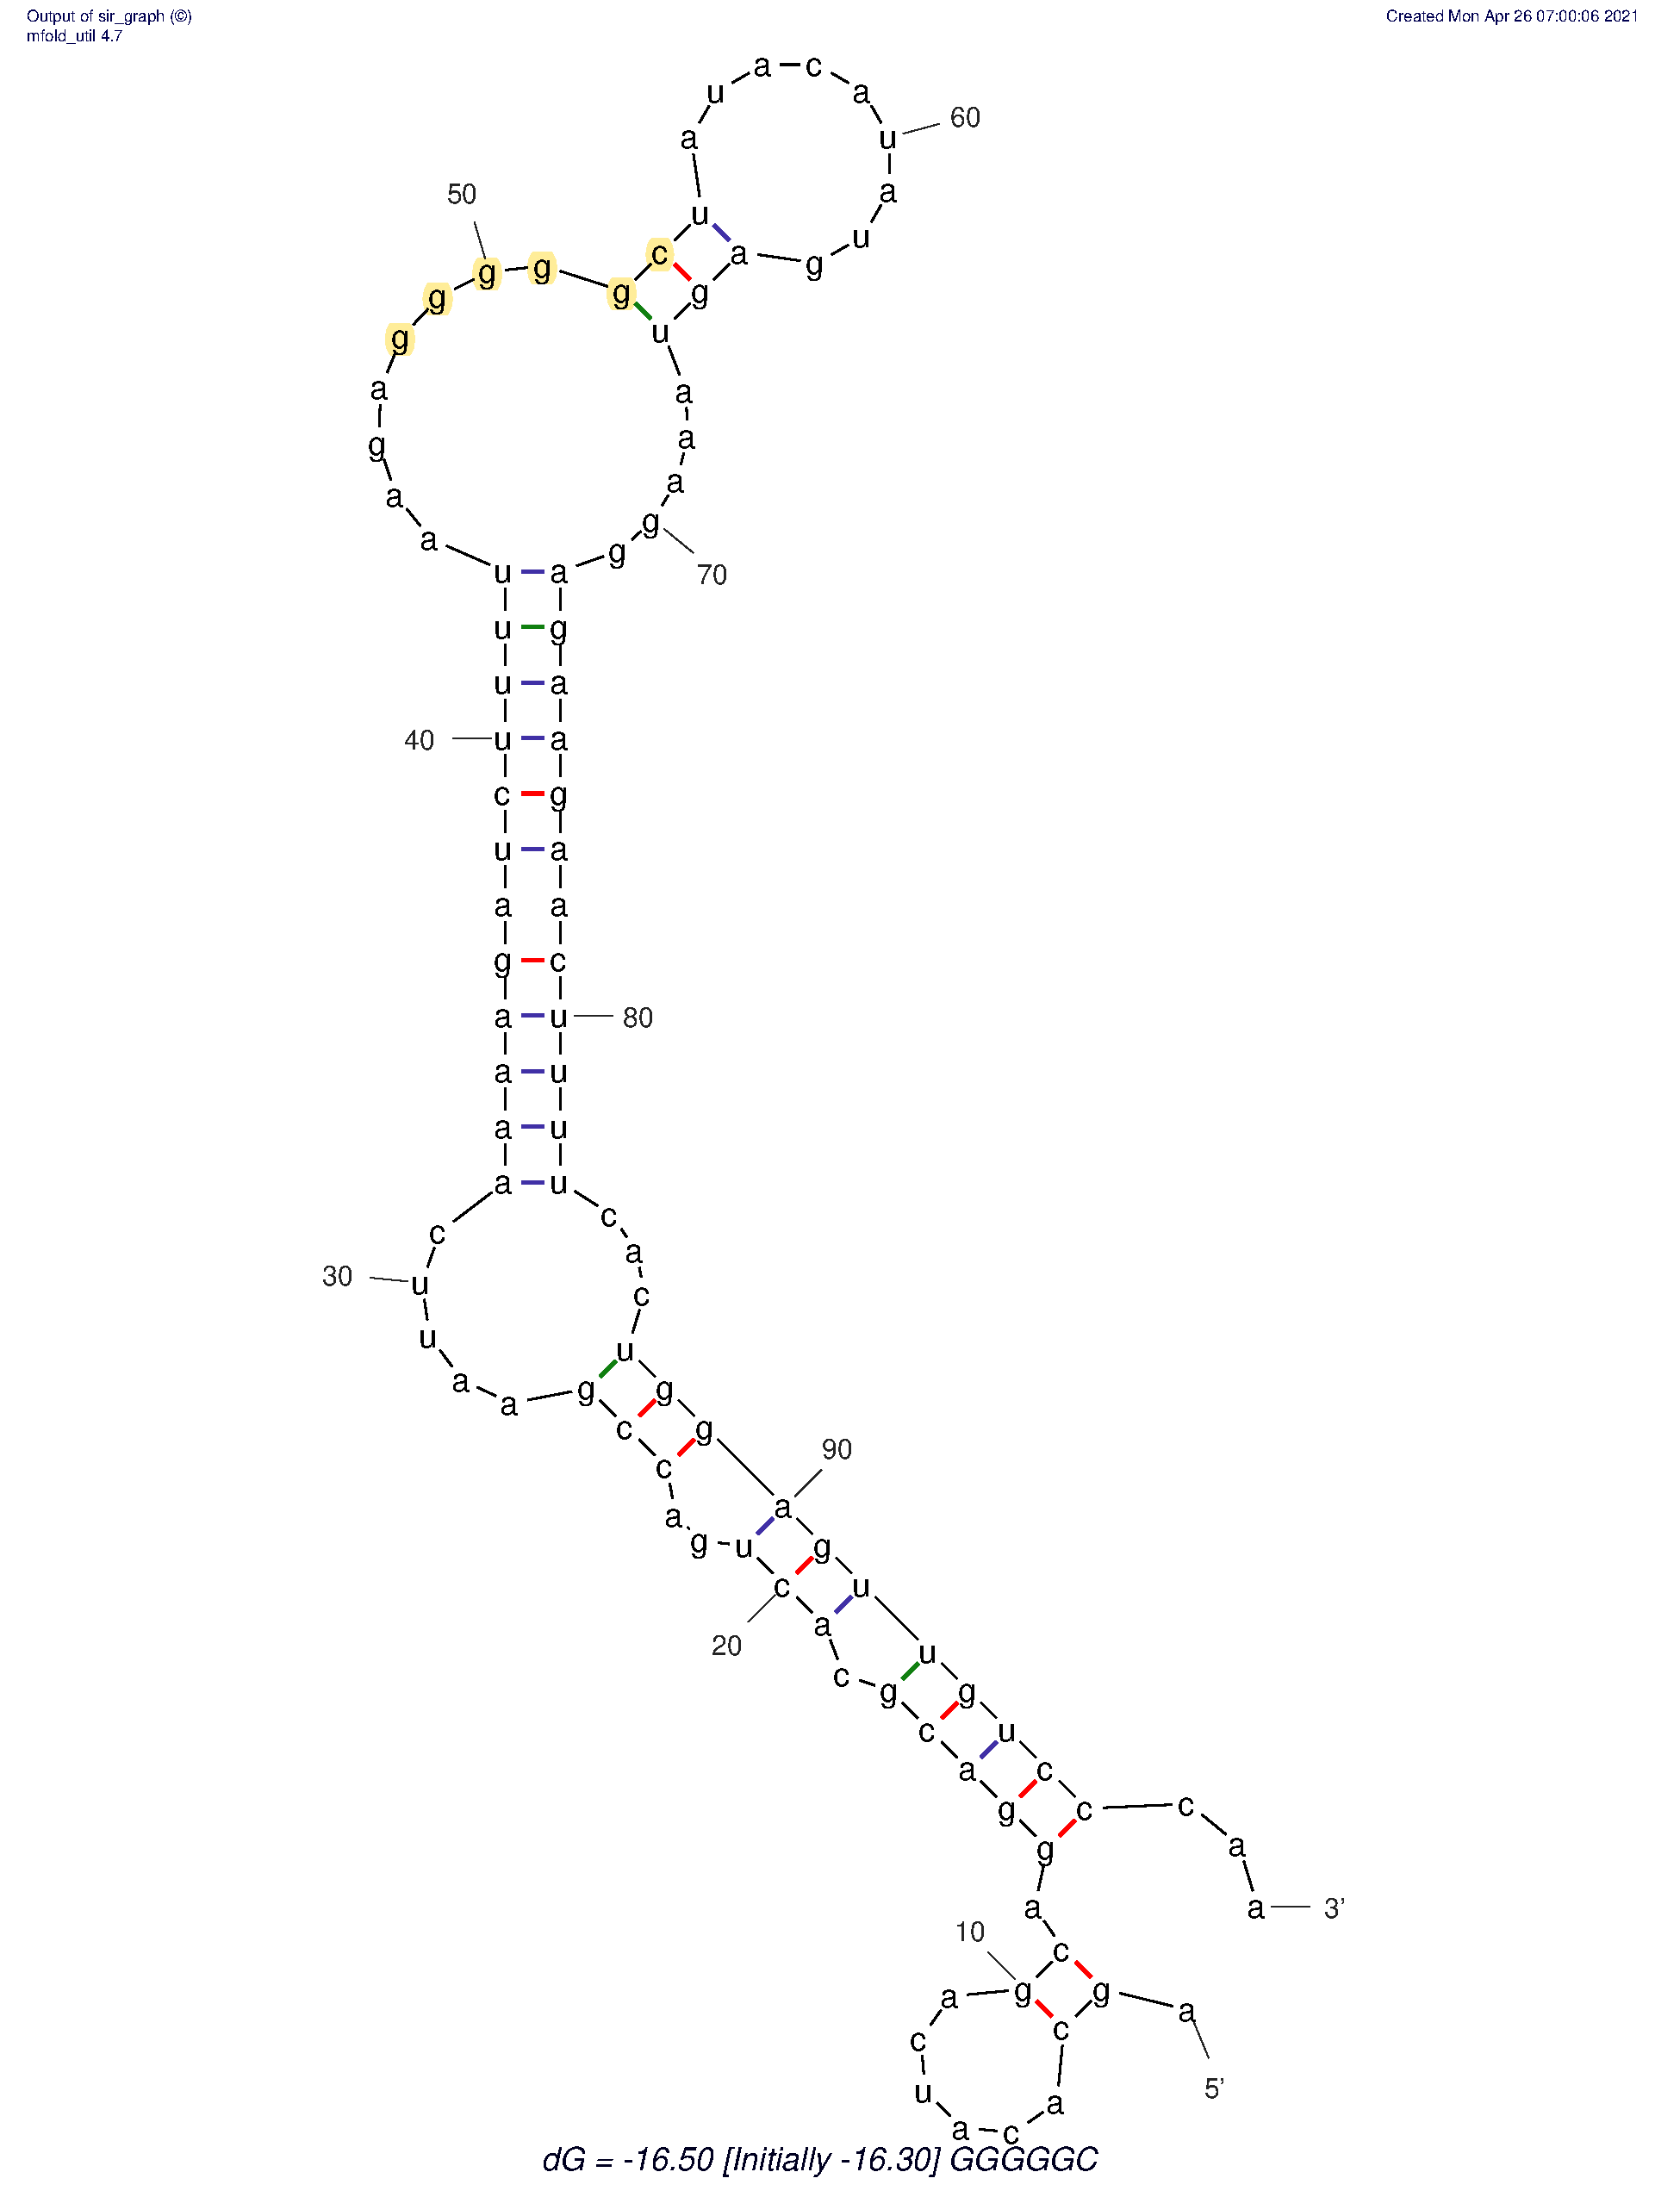
\includegraphics[scale=0.25]{plots/Supplementary/Structure GGGGGC.pdf}
         \caption{$y=3sinx$}
         \label{fig:GGGGGC}
     \end{subfigure}
     \vskip\baselineskip
     \begin{subfigure}[b]{0.49\textwidth}
         \centering
         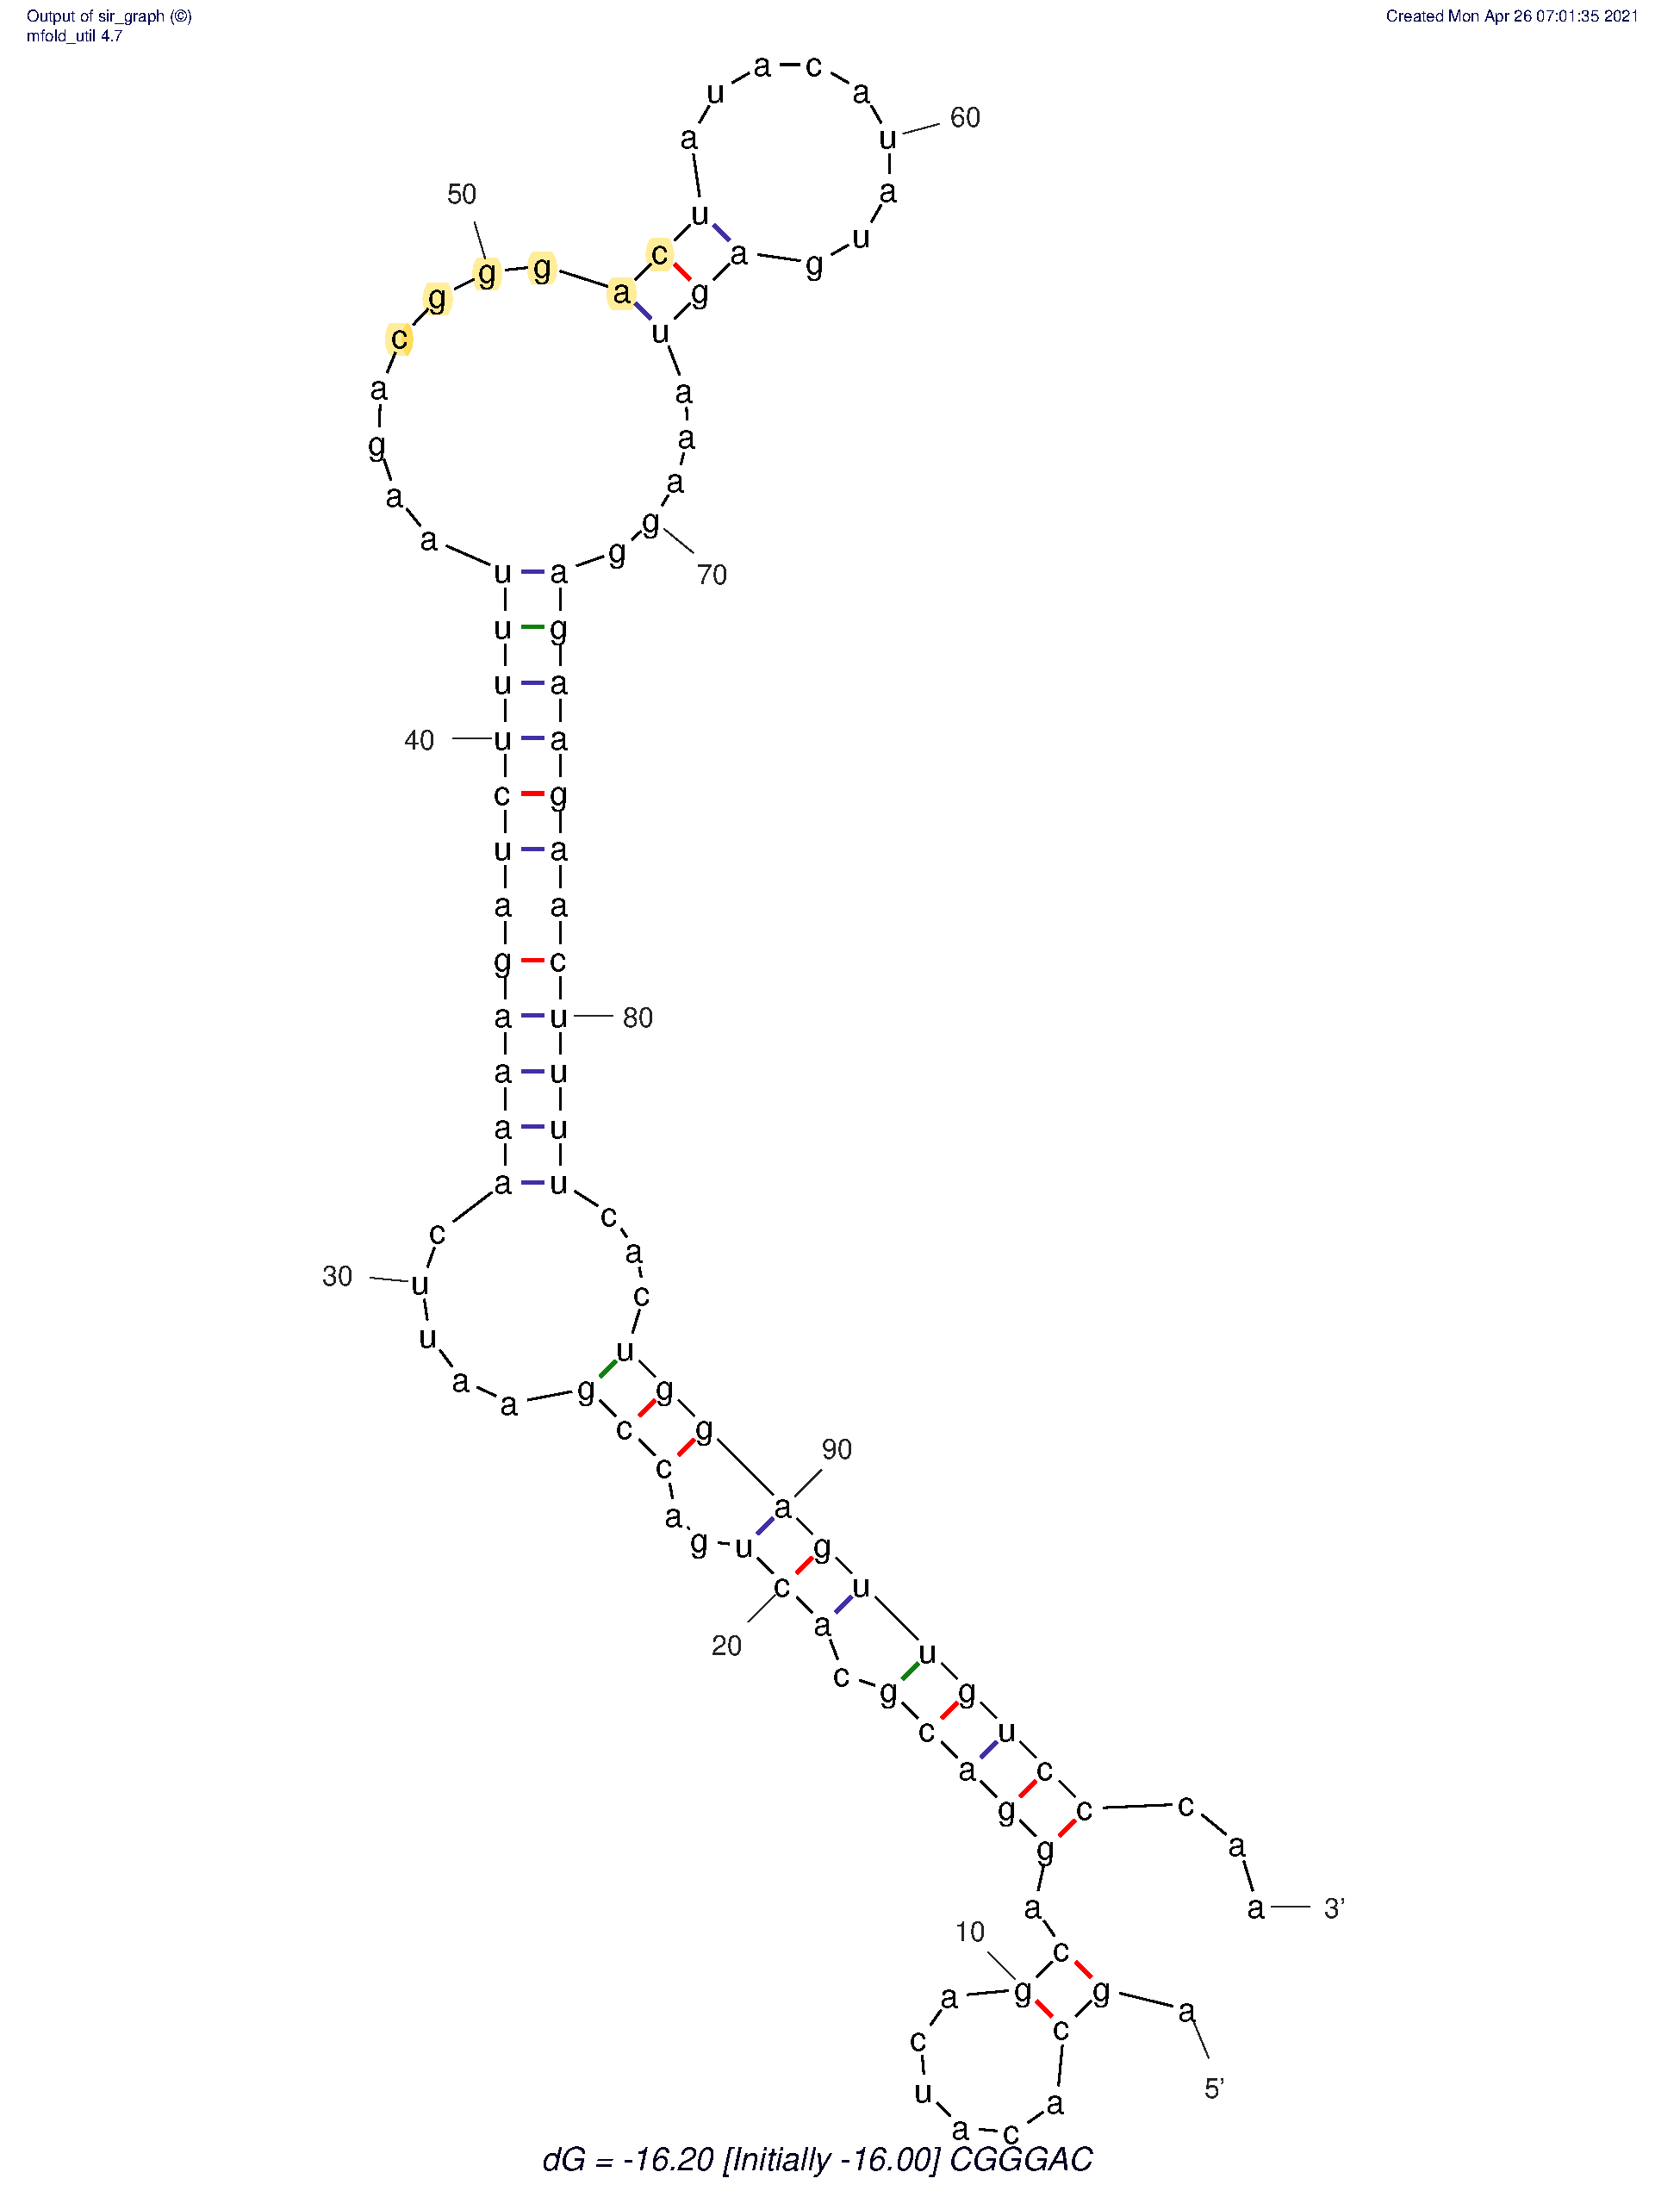
\includegraphics[scale=0.25]{plots/Supplementary/Structure CGGGAC.pdf}
         \caption{$y=5/x$}
         \label{fig:CGGGAC}
     \end{subfigure}
     \hfill
     \begin{subfigure}[b]{0.49\textwidth}
         \centering
         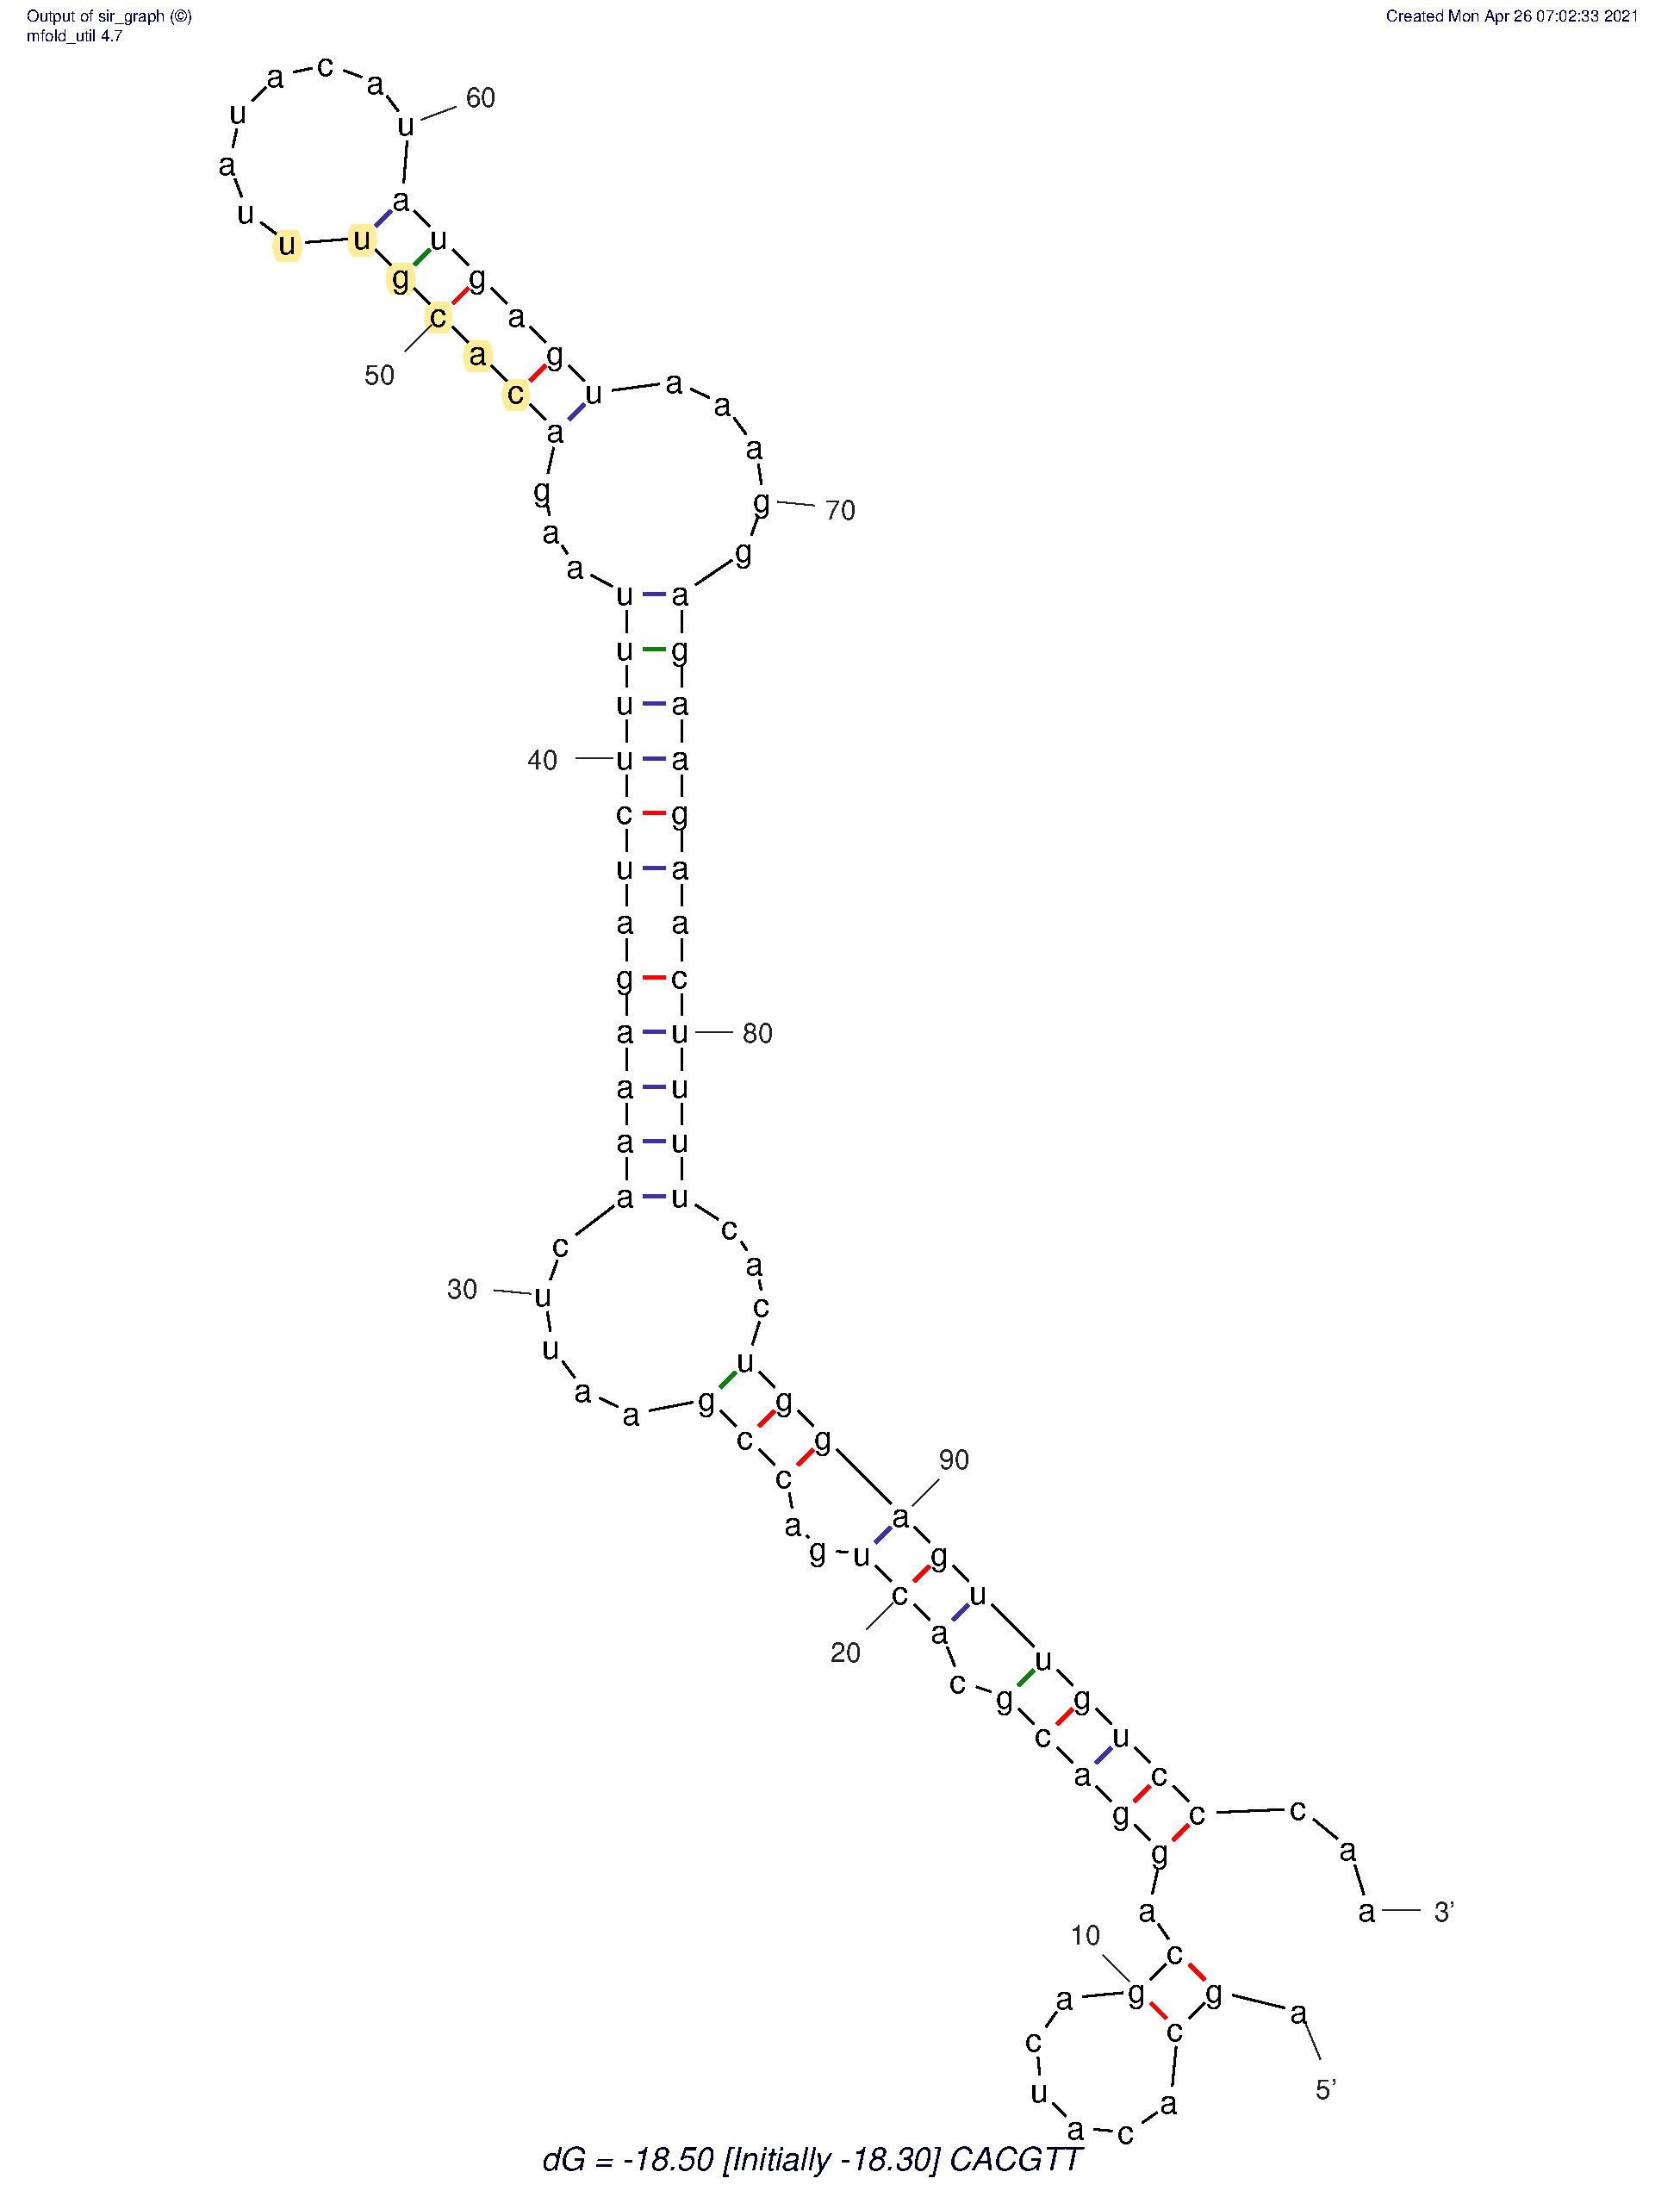
\includegraphics[scale=0.25]{plots/Supplementary/Structure CACGTT.pdf}
         \caption{$y=5/x$}
         \label{fig:CACGTT}
     \end{subfigure}
        \caption{\textbf{Folding predictionds for four different RBS.} Here we show the predicted, energetically most favourable structures for four of our RBS with the following cores: GGGGGG, GGGGGC, CGGGAC, CACGTT and their immediate upstream and downstream background sequence. There is no discerbile and consistent difference between strong ones (the first two) and weak ones (the last two).}
        \label{fig:structures}
\end{figure}


\end{document}
